% !TeX spellcheck = de_DE


\chapter{Einleitung}
	Die Veranstaltung "Data Mining und Maschinelles Lernen" behandelt, ebenso wie diese Zusammenfassung, den Teilbereich des maschinellen Lernens der künstlichen Intelligenz. Dabei werden Algorithmen entwickelt, durch die ein Computer sich selbstständig verbessert. Ein Teilgebiet dieses maschinellen Lernens ist das \emph{tiefe Lernen} (DL, für \emph{Deep Learning}), bei dem tiefe künstliche neuronale Netzwerke genutzt werden (dies wird im \autoref{c:deepLearning} näher behandelt). Dieser Zusammenhang ist in \autoref{fig:aiMlDl} dargestellt.

	Diese Zusammenfassung wird in die folgenden Bereiche einführen: k-Nächste Nachbarn, Lineare Modelle und Funktionsapproximation, Modellselektion und Evaluierung, Entscheidungsbäume, Ensemble-Methoden, Naive Bayes und Bayes-Netzwerke, die Stützvektormethode, Clusteranalyse und Assoziationsregeln und (Tiefe) Neuronale Netzwerke. Viele andere Bereiche werden allerdings auch nicht abgedeckt, \bspw Variational Learning, Details des Deep Learning, Gaussian Processes, Graphische Modelle, Kausalität, \dots Diese Inhalte sind zu Teilen in den Zusammenfassungen für die Kurse "Statistical Machine Learning", "Probabilistic Graphical Models" (noch nicht verfügbar, voraussichtlich im Wintersemester 2021/22), "Statistical Relational AI" (noch nicht verfügbar, voraussichtlich im Wintersemester 2021/22) sowie "Deep Learning: Architectures and Methods" (bald verfügbar) zu finden.

	\begin{figure}
		\centering
		\begin{tikzpicture}[align = center]
			\node (dl) {Tiefes \\ Lernen};
			\node [right = 1 of dl] (ml) {Maschinelles \\ Lernen};
			\node [right = 1 of ml] (ai) {Künstliche Intelligenz};

			\path (dl) -- coordinate(needle) (ml);

			\node [draw, ellipse, minimum height = 1.5cm, minimum width = 2cm] at (dl) {};
			\node [draw, ellipse, minimum height = 3cm, minimum width = 7cm] at (needle) {};
			\node [draw, ellipse, minimum height = 5cm, minimum width = 13cm] at (ml) {};
		\end{tikzpicture}
		\caption{Zusammenhang von künstlicher Intelligenz, maschinellem Lernen und tiefem Lernen.}
		\label{fig:aiMlDl}
	\end{figure}

	\section{Geschichte}
		Im Gegensatz zu den meisten Vermutungen hat die künstliche Intelligenz bereits eine lange Vergangenheit:
		\begin{description}[leftmargin = 2cm]
			\item[1950er] Geburt der künstlichen Intelligenz
			\item[1960er] Ära der Perzeptrons
			\item[1970er] Erster KI-Winter
			\item[1980er] Ära der Expertensysteme
			\item[1990er] Zweiter KI-Winter
			\item[2000er] Ära des statistischen maschinellen Lernens
			\item[2000er] Ära des tiefen Lernens
		\end{description}
		Das Perzeptron, welches im folgenden Abschnitt vorgestellt wird, hat die ersten großen Ergebnisse in der KI-Forschung produziert. Es hat zwar eine sehr mächtige Vorhersagekraft, es gibt jedoch Probleme, die nicht mit einem Perzeptron lösbar sind (Minsky, 1969). Diese Tatsache hat anschließend zu dem ersten KI-Winter geführt, in dem wenig geforscht wurde und das öffentliche Interesse abgeebbt ist. Gefolgt ist die Ära der Expertensysteme, Fall- und Regal-basierte KI-Systeme, die durch einen Menschen und logisches Schlussfolgern erstellt wurden. Jedoch haben auch diese Systeme zu viel versprochen und das öffentliche Interesse ist schnell abgeebbt.

		Nun betrat das moderne maschinelle Lernen mit dem \emph{statistischen} maschinellen Lernen das Feld, welches durch komplizierte statistische Modelle angetrieben und motiviert wurde. Die Ergebnisse haben sehr viele Erfolge gebracht, es gab jedoch kein großes Pressecho. Dies könnte unter anderem daher kommen, dass der Grundsatz der Forschung quantitative und messbare Ergebnisse waren und keine großen Ansprüche zur "Intelligenz" gestellt wurden. Darauf folgte die Ära des tiefen Lernens, also neuronale Netzwerke mit "vielen" Schichten, welches ein große Aufmerksamkeit von der Presse und Politik bekommt.

		\subsection{Das Perzeptron}
			Das von Frank Rosenblatt entwickelte \emph{Perzeptron} war das erste Modell, welches durch das menschliche Gehirn motiviert war, ein künstliches neuronales Netzwerk. Dabei werden viele kleine und einfache Einheiten (Neuronen) zu einem größeren Modell verbunden und das Lernen findet durch Anpassung der Verbindungsstärken (Synapsen) und -gewichten statt. Eine Darstellung eines solchen Perzeptrons ist in \autoref{fig:perceptron} gegeben. Dabei werden die Eingaben in der Neuronenschicht gewichtet und die Neuronen \emph{feuern}. Diese Ausgabe wird anschließend an das Ausgabeneuron weitergegeben, welches die \emph{Aktivierungen} akkumuliert und, sofern der akkumulierte Wert über einen gewissen Schwellenwert liegt, feuert. So kann eine binäre Klassifikation durchgeführt werden.

			Zum trainieren eines Perzeptrons werden bekannte Daten verwendet, in das Perzeptron eingegeben und die vorhergesagten Ergebnisse mit den echten verglichen. War die Vorhersage korrekt, wird nicht geändert. War die Vorhersage jedoch falsch, so werden die Verbindungsstärken so geändert, dass das Richtige vorhergesagt wird. Dies wird so lange wiederholt, bis keine Fehler mehr gemacht werden.

			Mit dem Wechsel zu tiefem Lernen werden diese einschichtigen nicht mehr verwendet, sondern es werden mehrere Neuronenschichten verwendet, die aufeinander Aufbauen (in \autoref{fig:mlp} in ein solches Netzwerk gezeigt). Neben der Nachteile des höheren Speicherverbrauchs, mehr benötigter Rechenkraft und der Anforderung an mehr Daten haben solche Modelle den großen Vorteil, dass sie eine deutlich höhere Vorhersagekraft besitzen.

			\begin{figure}
				\centering
				\begin{tikzpicture}[->]
					\node [input neuron] (a) {};
					\node [input neuron, below = 0.1 of a] (b) {};
					\node [input neuron, below = 0.1 of b] (c) {};
					\node [input neuron, below = 0.1 of c] (d) {};
					\node [input neuron, below = 0.1 of d] (e) {};

					\node [left = 2 of c] (I) {Input};

					\node [output neuron, right = 2 of c] (o) {};
					\node [right = 1 of o] (O) {Output};

					\draw (a) to[bend left = 10] (o);
					\draw (b) to[bend left = 5] (o);
					\draw (c) to (o);
					\draw (d) to[bend right = 5] (o);
					\draw (e) to[bend right = 10] (o);

					\draw (I) to[bend left = 10] (a);
					\draw (I) to[bend left = 5] (b);
					\draw (I) to (c);
					\draw (I) to[bend right = 5] (d);
					\draw (I) to[bend right = 10] (e);

					\draw (o) to (O);
				\end{tikzpicture}
				\caption{Darstellung eines einschichtigen Perzeptrons.}
				\label{fig:perceptron}
			\end{figure}

			\begin{figure}
				\centering
				\begin{tikzpicture}
					\node [input neuron] (a) {};
					\node [input neuron, below = 0.1 of a] (b) {};
					\node [input neuron, below = 0.1 of b] (c) {};
					\node [input neuron, below = 0.1 of c] (d) {};
					\node [input neuron, below = 0.1 of d] (e) {};

					\node [neuron, right = 1.5 of a] (l11) {};
					\node [neuron, right = 1.5 of b] (l12) {};
					\node [neuron, right = 1.5 of c] (l13) {};
					\node [neuron, right = 1.5 of d] (l14) {};
					\node [neuron, right = 1.5 of e] (l15) {};

					\node [neuron, right = 1.5 of l11] (l21) {};
					\node [neuron, right = 1.5 of l12] (l22) {};
					\node [neuron, right = 1.5 of l13] (l23) {};
					\node [neuron, right = 1.5 of l14] (l24) {};
					\node [neuron, right = 1.5 of l15] (l25) {};

					\node [neuron, right = 1.5 of l21] (l31) {};
					\node [neuron, right = 1.5 of l22] (l32) {};
					\node [neuron, right = 1.5 of l23] (l33) {};
					\node [neuron, right = 1.5 of l24] (l34) {};
					\node [neuron, right = 1.5 of l25] (l35) {};

					\node [output neuron, right = 1 of l33] (o) {};

					\draw (l31) to (o);
					\draw (l32) to (o);
					\draw (l33) to (o);
					\draw (l34) to (o);
					\draw (l35) to (o);

					\draw (a) to (l11);
					\draw (a) to (l12);
					\draw (a) to (l13);
					\draw (a) to (l14);
					\draw (a) to (l15);
					\draw (b) to (l11);
					\draw (b) to (l12);
					\draw (b) to (l13);
					\draw (b) to (l14);
					\draw (b) to (l15);
					\draw (c) to (l11);
					\draw (c) to (l12);
					\draw (c) to (l13);
					\draw (c) to (l14);
					\draw (c) to (l15);
					\draw (d) to (l11);
					\draw (d) to (l12);
					\draw (d) to (l13);
					\draw (d) to (l14);
					\draw (d) to (l15);
					\draw (e) to (l11);
					\draw (e) to (l12);
					\draw (e) to (l13);
					\draw (e) to (l14);
					\draw (e) to (l15);

					\draw (l11) to (l21);
					\draw (l11) to (l22);
					\draw (l11) to (l23);
					\draw (l11) to (l24);
					\draw (l11) to (l25);
					\draw (l12) to (l21);
					\draw (l12) to (l22);
					\draw (l12) to (l23);
					\draw (l12) to (l24);
					\draw (l12) to (l25);
					\draw (l13) to (l21);
					\draw (l13) to (l22);
					\draw (l13) to (l23);
					\draw (l13) to (l24);
					\draw (l13) to (l25);
					\draw (l14) to (l21);
					\draw (l14) to (l22);
					\draw (l14) to (l23);
					\draw (l14) to (l24);
					\draw (l14) to (l25);
					\draw (l15) to (l21);
					\draw (l15) to (l22);
					\draw (l15) to (l23);
					\draw (l15) to (l24);
					\draw (l15) to (l25);

					\draw (l21) to (l31);
					\draw (l21) to (l32);
					\draw (l21) to (l33);
					\draw (l21) to (l34);
					\draw (l21) to (l35);
					\draw (l22) to (l31);
					\draw (l22) to (l32);
					\draw (l22) to (l33);
					\draw (l22) to (l34);
					\draw (l22) to (l35);
					\draw (l23) to (l31);
					\draw (l23) to (l32);
					\draw (l23) to (l33);
					\draw (l23) to (l34);
					\draw (l23) to (l35);
					\draw (l24) to (l31);
					\draw (l24) to (l32);
					\draw (l24) to (l33);
					\draw (l24) to (l34);
					\draw (l24) to (l35);
					\draw (l25) to (l31);
					\draw (l25) to (l32);
					\draw (l25) to (l33);
					\draw (l25) to (l34);
					\draw (l25) to (l35);
				\end{tikzpicture}
				\caption{Darstellung eines mehrschichtigen Perzeptrons.}
				\label{fig:mlp}
			\end{figure}
		% end
	% end

	\section{KI Heute}
		Heute gibt es vier entscheidende Unterschiede zu vergangenen KI-Systemen:
		\begin{enumerate}
			\item Die Modelle sind größer.
				\begin{itemize}
					\item Früher wurden neuronale Netzwerke mit ein bis drei Schichten und hunderte bis tausende Neuronen verwendet.
					\item Heutige Modelle haben hunderte Schichten und hunderttausende Neuronen.
				\end{itemize}
			\item Es sind mehr Daten verfügbar.
				\begin{itemize}
					\item Früher waren tausende Bilder, hunderte Stunden Audiomaterial und hunderttausende Wörter verfügbar.
					\item Heute sind es Milliarden Bilder, Milliarden Stunden Audiomaterial und hunderte Milliarden Wörter.
					\item Diese Daten werden dabei in vielen großen Firmen gesammelt, \bspw hat YouTube mehr als zehn Milliarden Videos, Alibaba tätigt mehr als zwölf Milliarden Verkäufe pro Jahr, Facebook-Nutzer laden hunderte Milliarden Bilder pro Jahr hoch und Google kennt mehr als hundert Billionen Webseiten.
				\end{itemize}
			\item Heute Computer sind Leistungsfähiger.
				\begin{itemize}
					\item Früher konnte eine CPU \ca eine Millionen Operationen pro Sekunde ausführen und es gab keine GPUs.
					\item Heutige CPUs können mehr als eine Billionen Operationen pro Sekunde und heutige GPUs können mehr als zehn Billionen Operationen pro Sekunde ausführen.
				\end{itemize}
			\item Die Systeme funktionieren und lösen viele Aufgaben.
		\end{enumerate}
		Dabei ist der Hauptmotor der künstlichen Intelligenz aktuell das maschinelle Lernen.
	% end

	\section{Was ist Maschinelles Lernen?}
		\emph{Maschinelles Lernen} ist die Automatisierung von Automatisierung, es werden Teile des Computers so programmiert, dass sie sich anschließend selbstständig "programmieren". Das ist nötig, da das Schreiben von Software oftmals der Flaschenhals in der Entwicklung ist, da die Daten so schnell mehr werden. Es ist also klug, die Daten zu nutzen, um die Software selbst zu erstellen. Im Gegensatz zur traditionellen Programmierung werden also keine Ausgaben durch ein Programm erstellt, sondern es wird ein Programm aus Ausgaben erstellen (siehe \autoref{fig:traditionalVsMl}). Die Entwicklung von ML-Komponenten ist dabei ein Kreislauf, dargestellt in \autoref{fig:mlPipeline}.

		Anwendungsgebiete von maschinellem Lernen sind beispielsweise Websuche, Computational Biologie/Cognitive Science/Social Science/\dots, Finanzwelt, E-Commerce, Robotik, Debugging, Industrie 4.0 und viele mehr.

		\begin{figure}
			\centering
			\begin{subfigure}{0.49\linewidth}
				\centering
				\begin{tikzpicture}
					\node [draw, rectangle, minimum height = 1cm, minimum width = 2.5cm] (a) {Computer};
					\coordinate [above = 0.3 of a.west] (b);
					\coordinate [below = 0.3 of a.west] (c);
					\node [left = 0.75 of b] (d) {Daten};
					\node [left = 0.75 of c] (e) {Programm};
					\node [right = 0.75 of a.east] (f) {Ausgabe};
					\draw [->] (d) to (b);
					\draw [->] (e) to (c);
					\draw [->] (a.east) to (f);
				\end{tikzpicture}
				\caption{Traditionelle Programmierung}
			\end{subfigure}
			~
			\begin{subfigure}{0.49\linewidth}
				\centering
				\begin{tikzpicture}
					\node [draw, rectangle, minimum height = 1cm, minimum width = 2.5cm] (a) {Computer};
					\coordinate [above = 0.3 of a.west] (b);
					\coordinate [below = 0.3 of a.west] (c);
					\node [left = 0.75 of b] (d) {Daten};
					\node [left = 0.75 of c] (e) {Ausgabe};
					\node [right = 0.75 of a.east] (f) {Programm};
					\draw [->] (d) to (b);
					\draw [->] (e) to (c);
					\draw [->] (a.east) to (f);
				\end{tikzpicture}
				\caption{Maschinelles Lernen}
			\end{subfigure}
			\caption{Traditionelle Programmierung (links) im Vergleich zu maschinellem Lernen (rechts).}
			\label{fig:traditionalVsMl}
		\end{figure}

		\begin{figure}
			\centering
			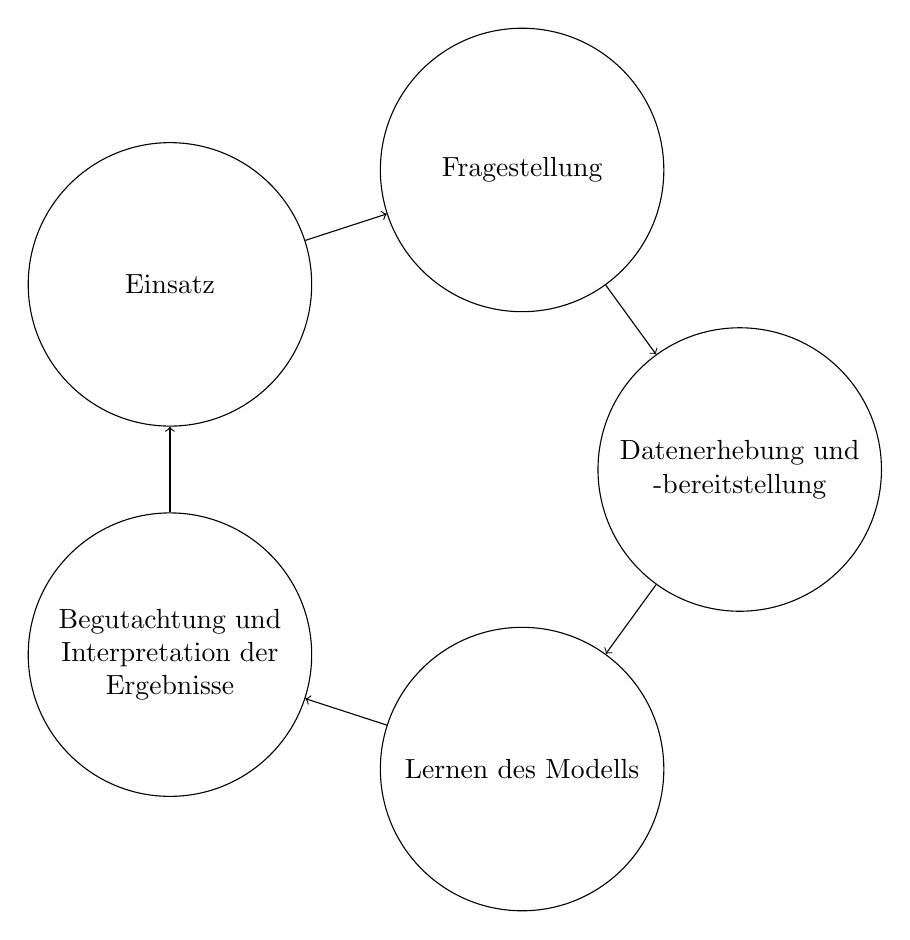
\begin{tikzpicture}[->, align = center, every node/.style = { draw, circle, minimum height = 2cm, minimum width = 3.6cm }]
				\node (a) at (-288:4cm) {Fragestellung};
				\node (b) at (-  0:4cm) {Datenerhebung und \\ -bereitstellung};
				\node (c) at (- 72:4cm) {Lernen des Modells};
				\node (d) at (-144:4cm) {Begutachtung und \\ Interpretation der \\ Ergebnisse};
				\node (e) at (-216:4cm) {Einsatz};
				\draw (a) to (b);
				\draw (b) to (c);
				\draw (c) to (d);
				\draw (d) to (e);
				\draw (e) to (a);
			\end{tikzpicture}
			\caption{Kreislauf der Erstellung von ML-Komponenten.}
			\label{fig:mlPipeline}
		\end{figure}

		\subsection{Kurzgefasst}
			Im Bereich des maschinellen Lernens gibt es viele tausende Algorithmen und hunderte neue Algorithmen pro Jahr. Dabei adressiert jeder Algorithmus die folgenden drei Fragestellungen:
			\begin{enumerate}
				\item Wie wird das Modell \emph{repräsentiert}? \\
					Entscheidungsbäume, Regeln/logische Programme, Instanzen, Probabilistische Graphische Modelle, Neuronale Netzwerke, Stützvektormaschinen, Ensembles, \dots
				\item Wie wird das Modell \emph{optimiert}? \\
					Kombinatorische Optimierung (\zB Greedy-Suche), Konvexe und nichtlineare Optimierung (\zB Gradientenabstieg), Optimierung unter Randbedingungen (\zB lineare Programmierung), \dots
				\item Wie wird das Modell \emph{evaluiert} und \emph{beurteilt}? \\
					Korrektklassifikationsrate (Accuracy), Genauigkeit (Precision) und Trefferquote (Recall), Quadrierter Fehler, Likelihood, A-Posteriori Wahrscheinlichkeit, Kosten/Nutzen, Margin, Entropie, KL-Divergenz, \dots
			\end{enumerate}

			Dabei gibt es vier große Kategorien des maschinellen Lernens:
			\begin{description}
				\item[Überwacht (Induktiv)] Die Trainingsdaten erhalten neben Eingaben auch gewünschten Ausgaben. \\
					Englisch: \emph{Supervised Learning}
				\item[Unüberwacht] Die Trainingsdaten erhalten nur Eingaben und \emph{keine} Ausgaben. \\
					Englisch: \emph{Unsupervised Learning}
				\item[Teilweise Überwacht] Die Trainingsdaten \emph{einige} gewünschte Ausgaben, aber nicht alle. \\
					Englisch: \emph{Semi-supervised Learning}
				\item[Verstärkend] Der Algorithmus wird belohnt nachdem er eine Reihe an Aktionen ausgeführt hat und die Belohnung wird maximiert. \\
					Englisch: \emph{Reinforcement Learning}
			\end{description}
			Die Bereiche des überwachten und unüberwachten Lernens lassen sich dann noch weiter einordnen, was in \autoref{fig:mlTypes} gezeigt ist.

			\begin{figure}
				\centering
				\begin{tikzpicture}[
							->,
							align = center,
							block/.style = {
								draw,
								rectangle,
								minimum width = 3.25cm,
								minimum height = 1.5cm,
							},
								small/.style = {
								minimum height = 0.8cm,
							},
						]
					\node [block] (ml) {Maschinelles \\ Lernen};
					\node [block, right = 2 of ml, yshift = +3cm] (supervised) {Überwachtes \\ Lernen};
					\node [block, right = 2 of ml] (unsupervised) {Unüberwachtes \\ Lernen};
					\node [block, right = 2 of ml, yshift = -3cm] (rl) {Verstärkendes \\ Lernen};

					\node [block, small, right = 2 of supervised, yshift = +0.75cm] (class) {Klassifikation};
					\node [block, small, right = 2 of supervised, yshift = -0.75cm] (regress) {Regression};

					\node [block, small, right = 2 of unsupervised, yshift = +0.75cm] (dimred) {Dim.-Reduktion};
					\node [block, small, right = 2 of unsupervised, yshift = -0.75cm] (cluster) {Clustering};

					\draw (ml.east) to [bend right, out = -45+10, in = +180-45] (supervised.west);
					\draw (ml.east) to (unsupervised.west);
					\draw (ml.east) to [bend left,  out = +45-10, in = -180+45] (rl.west);

					\draw (supervised.east) to [bend right, out = -45+30, in = +180-45+30] (class.west);
					\draw (supervised.east) to [bend left,  out = +45-30, in = -180+45-30] (regress.west);

					\draw (unsupervised.east) to [bend right, out = -45+30, in = +180-45+30] (dimred.west);
					\draw (unsupervised.east) to [bend left,  out = +45-30, in = -180+45-30] (cluster.west);
				\end{tikzpicture}
				\caption{Arten des maschinellen Lernens.}
				\label{fig:mlTypes}
			\end{figure}
		% end
	% end
% end

\chapter{Grundlagen}
	Dieses Kapitel behandelt einige Grundlagen, die für das maschinelle Lernen benötigt werden.

	\section{CRISP-DM: Verlaufsmodell des Data Mining}
		Die Schritte des CRISP-DM (Cross-Industry Standard Process for Data Mining), dem Verlaufsmodell des Data Mining, sind:
		\begin{description}
			\item[Problem Verstehen] Analyseziele, Situationsbewertung, Datenanalyseziele, Projektplan
			\item[Daten Verstehen] Sammeln, Beschreiben, Untersuchen, Qualität von Rohdaten
			\item[Daten Aufbereiten] Ein- und Ausschluss, Bereinigung, Transformation von Variablen
			\item[Modellierung] Methoden- und Testdesignwahl, Schätzung, Modellqualität
			\item[Evaluierung] Modell akzeptieren, Prozess überprüfen, Nächste Schritte festlegen
			\item[Nachbereitung] Anwendungs- und Wartungsplan, Präsentation, Bericht
		\end{description}
		Diese Schritte sind grafisch in \autoref{fig:crisp} dargestellt.

		\begin{figure}
			\centering
			\includegraphics[width=0.5\linewidth]{img/crisp-dm}
			\caption{Grafische Übersicht über das CRISP-DM. \\ Autor: Kenneth Jensen \\ Lizenz: CC BY-SA 3.0 \\ Quelle: Wikipedia Commons, Datei CRISP-DM\_Process\_Diagram.png}
			\label{fig:crisp}
		\end{figure}
	% end

	\section{Klassifikation und Regression}
		Bei überwachtem maschinellen Lernen wird jeder Beobachtung \(\vec{x}\) ein Label \(y\) zugeordnet, \dh die Datenpunkte sind gegeben als \( (\vec{x}, y) \in X \times Y \), wobei \(X\) und \(Y\) die Mengen aller möglichen Beobachtungen/Labels sind. Im Teilbereich der \emph{Klassifikation} sind die Labels diskret, \dh es wird eine \emph{qualitative} Beschreibung gesucht. Im Gegensatz dazu steht die \emph{Regression}, bei der die Labels kontinuierlich sind und eine \emph{quantitative} Beschreibung gesucht wird.

		Das Ziel ist immer eine \emph{wahre Funktion} \( f : X \to Y \) zu finden, die für alle Eingaben \( \vec{x} \in X \) und Labels \( y \in Y \) den korrekten Wert liefert, \dh \( f(\vec{x}) = y \). Das Problem ist im Allgemeinen, dass nur eine Teilmenge aller Beobachtungen gegeben ist, die \emph{Trainingsdaten}. Auf Basis dieser Trainingsdaten wird nun eine Annäherung \( \hat{f} \) an die wahre Funktion \(f\) gesucht, welche als \emph{Modell} bezeichnet wird. Wurde ein Modell gefunden, so liefert dieses über
		\begin{equation}
			\hat{y} = \hat{f}(\vec{x})
		\end{equation}
		eine \emph{Vorhersage} \( \hat{y} \in Y \) für ein Datum \( \vec{x} \in X \).

		Dabei kann zur Klassifikation sowohl ein spezifisches als auch ein Regressionsmodell genutzt werden. Es können zum Beispiel alle Werte oberhalb eines Schwellenwertes \(\theta\) der einen und alle anderen Werte der anderen Klasse (im Fall von binären Klassifikationsproblemen) zugeordnet werden:
		\begin{equation}
			\hat{y} =
				\begin{cases}
					+1 & \text{falls } \hat{f}(\vec{x}) \geq \theta \\
					-1 & \text{sonst}
				\end{cases}
		\end{equation}
		Diese Art der Zuordnung ist nur eine Möglichkeit, ein Regressionsmodell als Klassifikationsmodell zu nutzen. Eine weitere ist \zB die logistische Regression, siehe \autoref{sec:logisticRegression}.
	% end

	\section{Statistik}
		In diesem Abschnitt werden benötigte grundlegenden Begriffe der Statistik eingeführt.

		\subsection{Erwartungswert, Varianz und Standardabweichung}
			Für eine diskrete Zufallsvariable \(X\) mit Werten \( x_i \) ist der \emph{Erwartungswert} gegeben durch
			\begin{equation}
				\E[X] = \sum_i x_i P(X = x_i).
			\end{equation}
			Für eine kontinuierliche Zufallsvariable \(X\) mit der Wahrscheinlichkeitsdichte \(p\) wird die Summe durch ein Integral ersetzt:
			\begin{equation}
				\E[X] = \int_{-\infty}^{\infty} \! x f(x) \dd{x}
			\end{equation}
			Oftmals werden dabei die Integrationsgrenzen weggelassen.

			Eine wichtige Eigenschaft des Erwartungswerts ist, dass dieser linear ist, \dh es gilt
			\begin{equation}
				\E[aX + bY] = a \E[X] + b \E[Y]
			\end{equation}
			für zwei Zufallsvariablen \(X\), \(Y\) und skalare \(a\), \(b\). Sind die Zufallsvariablen \(X\), \(Y\) stochastisch unabhängig, so gilt
			\begin{equation}
				\E[XY] = \E[X] \E[Y]
			\end{equation}

			Die \emph{Varianz} einer Zufallsvariablen ist gegeben durch die mittlere quadratische Abweichung vom Mittelwert,
			\begin{equation}
				\Var[X] = \E\big[ (X - \E[X])^2 \big].
			\end{equation}
			Sie wird oft auch mit \(\sigma^2\) bezeichnet. Die \emph{Standardabweichung} einer Zufallsvariable ist dann \(\sigma = \sqrt{\Var[X]}\). Nach dem \emph{Verschiebungssatz} gilt, wie einfach herzuleiten ist:
			\begin{equation}
				\Var[X] = \E\big[ (X - \E[X])^2 \big] = \E\big[ X^2 \big] - \big( \E[X] \big)^2.
			\end{equation}
		% end

		\subsection{Bias}
			\label{subsec:foundationsBias}

			Der \emph{Bias} eines Schätzers \(\hat{y}\) für eine Zufallsvariable \(Y\) bezeichnet die mittlere Verzerrung
			\begin{equation}
				\Bias[\hat{y}] = \E[Y - \hat{y}] = \E[Y] - \hat{y}
			\end{equation}
			des Schätzers. Ein Schätzer mit einem Bias von Null wird als \emph{Erwartungstreu} oder \emph{Unbiased} bezeichnet.

			Oftmals kann bei einem Schätzer nur entweder die Varianz oder der Bias reduziert werden, was als \emph{Bias-Varianz Trade-Off} bezeichnet wird.
		% end

		\subsection{Normalverteilung}
			Die \emph{Normalverteilung} (auch \emph{Gauß-Verteilung}) ist eine der wichtigsten Wahrscheinlichkeitsverteilungen in der Statistik. Dabei heißt eine Zufallsvariable \(X\) \emph{normalverteilt} mit Mittelwert \(\mu\) und Varianz \(\sigma^2\), wenn sie die Wahrscheinlichkeitsdichte
			\begin{equation}
				p(x) = \frac{1}{\sqrt{2 \pi \sigma^2}} \exp\bigg\{\!\! -\frac{1}{2} \frac{(x - \mu)^2}{\sigma^2} \bigg\}
			\end{equation}
			besitzt.
		% end

		\subsection{Bedingte Wahrscheinlichkeiten}
			Bedingte Wahrscheinlichkeiten, geschrieben \( P(X = x \given Y = y) \), beschreiben die Wahrscheinlichkeit einer Zufallsvariable \(X\) den Wert \(x\) anzunehmen, wenn eine andere Zufallsvariable \(Y\) den Wert \(y\) hat. Zufallsvariablen \(X\), \(Y\) heißen \emph{stochastisch unabhängig}, wenn \( P(X = x \given Y = y) = P(X = x) \) gilt. Im Allgemeinen gilt
			\begin{equation}
				P(X \given Y = y) = \frac{P(X = x, Y = y)}{P(Y = y)},
			\end{equation}
			wobei \( P(X = x, Y = y) \) die \emph{Verbundwahrscheinlichkeit} ist.
		% end

		\subsection{Bayes-Statistik}
			Eine der wichtigsten Formeln in der Statistik in die Bayes-Formel
			\begin{equation}
				p(x \given y) = \frac{p(y \given x) \, p(x)}{p(y)},
			\end{equation}
			die den Zusammenhang zwischen der Likelihood \( p(y \given x) \), der A-Priori Wahrscheinlichkeit \( p(x) \) und der A-Posteriori Wahrscheinlichkeit \( p(x \given y) \) beschreibt. Der Faktor \( p(y) \) dient dabei nur der Normalisierung, weshalb die Bayes-Formel oft auch als
			\begin{equation}
				p(x \given y) \propto p(y \given y) \, p(x)
			\end{equation}
			geschrieben wird.
		% end

		\subsection{Konfidenzintervalle}
			Ein \emph{Konfidenzintervall} ist ein Intervall \( [\ell, u] \), welches aus einer gegebenen Irrtumswahrscheinlichkeit \(\alpha\) erzeugt wird. Es gibt den Bereich an, in dem der Wert der Zufallsvariable mit Wahrscheinlichkeit \( 1 - \alpha \) liegt:
			\begin{equation}
				P(\ell \leq X \leq u) = 1 - \alpha
			\end{equation}
			Eine häufige Wahl ist die Bildung eines Konfidenzintervalls für den Erwartungswert. So können Aussagen wie "Mit \SI{90}{\percent} Wahrscheinlichkeit liegt der Mittelwert im Intervall \( [\ell, u] \)." getätigt werden (hier mit \( \alpha = 0.01 \)).

			Konfidenzintervalle sind ein mächtiges Werkzeug in der Bewertung von Verfahren, was in \autoref{c:trees} weiter behandelt wird.
		% end

		\subsection{Entropie}
			Die Entropie einer Wahrscheinlichkeitsverteilung \(P(X)\) gibt an, wie viel Informationsgehalt in dieser steckt. Für eine diskrete Zufallsvariable \(X\) mit den möglichen Werten \(\mathcal{X}\) wird die Entropie wie folgt berechnet:
			\begin{equation}
				H(X) = -\!\sum_{x \,\in\, \mathcal{X}} P(x) \,\log P(x)
			\end{equation}
			Für eine kontinuierliche Zufallsvariable \(X\) mit Wahrscheinlichkeitsdichte \(p(X)\) gilt
			\begin{equation}
				H(X) = -\!\int\! p(x) \,\log p(x) \dd{x}\!,
			\end{equation}
			wobei wie vorher beschrieben die Integrationsgrenzen zur Übersichtlichkeit weggelassen werden. Wird der Logarithmus zur Basis \num{2} verwendet, so kann die Entropie einer Verteilung auch als die Anzahl Bits angesehen werden, die mindestens zur Übertragung benötigt werden.

			\subparagraph{Beispiel}
				Es werden Nachrichten \(X\) mit den Werten \(a\), \(b\), \(c\) und \(d\) versendet. Eine Aufzeichnung des Netzwerkverlaufs stellt fest, dass die Nachrichten mit den folgenden Häufigkeiten gesendet werden:
				\begin{center}
					\begin{tabular}{c|c|c|c}
						\(a\) & \(b\) & \(c\) & \(d\) \\ \hline
						 25   &   7   &  14   &  54
					\end{tabular}
				\end{center}
				Bei einer Gesamtanzahl von \( 25 + 7 + 14 + 54 = 100 \) ergeben sich also die folgenden relativen Häufigkeiten, \bzw die folgende empirische Verteilung:
				\begin{equation}
					\begin{aligned}
						P(X = a) &= 25\% &
						P(X = b) &= 7\%  \\
						P(X = c) &= 14\% &
						P(X = d) &= 54\%
					\end{aligned}
				\end{equation}
				Der Informationsgehalt \( -\log_2 P(X) \) je Symbol ist:
				\begin{equation}
					\begin{aligned}
						-\log_2 P(X = a) &= 2      &
						-\log_2 P(X = a) &= 3.8365 \\
						-\log_2 P(X = a) &= 2.8365 &
						-\log_2 P(X = a) &= 0.888969
					\end{aligned}  \label{eq:entropyExampleInformation}
				\end{equation}
				Daraus ergibt sich die folgende Gesamtentropie:
				\begin{align}
					H(X)
						&= -\big(
								\begin{aligned}[t]
									 &\, \eqmakebox[entropyExample][l]{\(\displaystyle P(X = a)\)} \,\log P(X = a) \\
								   + &\, \eqmakebox[entropyExample][l]{\(\displaystyle P(X = b)\)} \,\log P(X = b) \\
								   + &\, \eqmakebox[entropyExample][l]{\(\displaystyle P(X = c)\)} \,\log P(X = c) \\
								   + &\, \eqmakebox[entropyExample][l]{\(\displaystyle P(X = d)\)} \,\log P(X = d) \quad\big)
								\end{aligned}
						\\
						&= 0.25 \cdot 2 + 0.007 \cdot 3.8365 + 0.14 \cdot 2.8365 + 0.54 \cdot 0.888969 \\
						&= 1.40401
				\end{align}
				Es werden also mindestens \num{2} Bits benötigt, um die Nachricht zu kodieren.

				An dem Informationsgehalt \eqref{eq:entropyExampleInformation} ist zu sehen, dass as Symbol \(d\) die wenigsten Informationen überträgt, da es am häufigsten vorkommt. Dies kann Interpretiert werden als "Überraschungseffekt" beim Empfänger: Kommt ein \(d\) an, ist dies nicht überraschen, da dies in \SI{54}{\%} der Fälle passiert. Kommt jedoch ein \(b\) an, ist dies sehr ungewöhnlich.
			% end
		% end
	% end
% end

\chapter{k-Nächste Nachbarn (kNN)}
	Im Allgemeinen können Verfahren des maschinellen Lernens in \emph{globale} und \emph{lokale} Modelle unterteilt werden: Lokale Modelle Klassifizieren einen Datenpunkt nur Anhand seiner Umgebung, globale Modelle hingegen finden ein global Gültiges Entscheidungskriterium, beispielsweise eine trennende Hyperebene. Das verfahren der \emph{k-Nächsten Nachbarn} (kNN) gehört zu den lokalen Modelle. Bei diesem Ansatz wird ein Beispiel anhand der \(k\) nächsten Nachbarn (nach irgendeiner Ähnlichkeitsmetrik) klassifiziert: Ein Datenpunkt gehört einer bestimmten Klasse an, wenn der Großteil der umliegenden Datenpunkte auch dieser Klasse angehören. Leicht formalisiert ergibt sich folgendes Vorgehen (wobei \( f(\cdot) \) die tatsächliche Kategorie beschreibt):
	\begin{enumerate}
		\item Berechne den Abstand zwischen dem Datenpunkt \( \vec{x}_\ast \) und jedem Trainingsdatenpunkt.
		\item Wähle die \(k\) nächsten Nachbarn \( \dotsrange{\vec{n}_1}{\vec{n}_k} \) bezüglich einem Ähnlichkeitsmaß \( \mathit{dist}(\vec{x}, \vec{y}) \).
		\item Berechne die Vorhersage \( A\big( \vec{x}_\ast;\, \dotsrange{f(\vec{n}_1)}{f(\vec{n}_k)} \big) \).
	\end{enumerate}
	Hier werden sofort einige Schwierigkeiten ersichtlich:
	\begin{itemize}
		\item Welches Ähnlichkeitsmaß \( \mathit{dits}(\cdot, \cdot) \) sollte verwendet werden?
		\item Wie viele Nachbarn \(k\) sollten verwendet werden?
		\item Was passiert, wenn die Werte der Nachbarn nicht überein stimmen oder es ein Unentschieden gibt?
		\item Wie kann die Suche effizient gestaltet werden?
	\end{itemize}

	\section{Ähnlichkeitsmaße}
		Wie bereits beschrieben ist ein Problem die Auswahl eines Ähnlichkeitsmaßes. Die zwei wichtigsten Eigenschaften des Ähnlichkeitsmaßes sind, dass dieses kleiner werden sollte, wenn zwei Datenpunkte sich ähnlicher sind und genau dann Null ist, wenn zwei Datenpunkte identisch sind. Eine Möglichkeit ist beispielsweise der euklidische Abstand
		\begin{equation}
			\mathit{dist}(\vec{x}, \vec{y}) = \lVert \vec{x} - \vec{y} \rVert_2 = \sqrt{\textstyle \sum_{i = 1}^{n} (x_i - y_i)^2}
		\end{equation}
		oder der Kosinus-Abstand
		\begin{equation}
			\mathit{dist}(\vec{x}, \vec{y}) = \cos(\vec{x}, \vec{y}) = \frac{\braket{\vec{x}}{\vec{y}}}{\lvert \vec{x} \rvert \, \lvert \vec{y} \rvert} = \frac{\sum_{i = 1}^{n} x_i y_i}{\sqrt{\sum_{i = 1}^{n} x_i^2} \, \sqrt{\sum_{i = 1}^{n} y_i^2}},
		\end{equation}
		welcher Invariant gegenüber Skalierungen der Vektoren ist. Andere Ähnlichkeitsmaße für binäre (0/1) Daten sind \zB:
		\begin{itemize}
			\item Matching Koeffizient:
		\end{itemize}
		\begin{equation}
			\lvert \vec{x} \cap \vec{y} \rvert
		\end{equation}
		\begin{itemize}
			\item Dice Koeffizient:
		\end{itemize}
		\begin{equation}
			\frac{2 \lvert \vec{x} \cap \vec{y} \rvert}{\lvert \vec{x} \rvert + \lvert \vec{y} \rvert}
		\end{equation}
		\begin{itemize}
			\item Jaccard Koeffizient.
		\end{itemize}
		\begin{equation}
			\frac{\lvert \vec{x} \cap \vec{y} \rvert}{\lvert \vec{x} \cup \vec{y} \rvert}
		\end{equation}
		\begin{itemize}
			\item Overlap Koeffizient:
		\end{itemize}
		\begin{equation}
			\frac{\lvert \vec{x} \cap \vec{y} \rvert}{\min \{ \lvert \vec{x} \rvert, \lvert \vec{y} \rvert \}}
		\end{equation}
		\begin{itemize}
			\item Kosinus:
		\end{itemize}
		\begin{equation}
			\frac{\lvert \vec{x} \cap \vec{y} \rvert}{\sqrt{\lvert \vec{x} \rvert} \, \sqrt{\lvert \vec{x} \rvert}}
		\end{equation}
		Dabei beschreibt \( \cap \) eine komponentenweise Und-Aggregation und \( \cup \) eine Oder-Aggregation:
		\begin{align}
			\begin{bmatrix}
				0 \\ 0 \\ 1 \\ 1
			\end{bmatrix}
			\cap
			\begin{bmatrix}
				0 \\ 1 \\ 0 \\ 1
			\end{bmatrix}
			&=
			\begin{bmatrix}
				0 \\ 0 \\ 0 \\ 1
			\end{bmatrix}
			&
			\begin{bmatrix}
				0 \\ 0 \\ 1 \\ 1
			\end{bmatrix}
			\cup
			\begin{bmatrix}
				0 \\ 1 \\ 0 \\ 1
			\end{bmatrix}
			&=
			\begin{bmatrix}
				0 \\ 1 \\ 1 \\ 1
			\end{bmatrix}
		\end{align}

		Trotz dieser vielen Ähnlichkeitsmaße ist es im Allgemeinen aber sehr schwer zu entscheiden, ob sich zwei Datenpunkte (\zB Bilder) ähnlich sind -- die Bedeutung von "ähnlich" scheint an dieser Stelle eher ein philosophisches Problem zu sein, im maschinellen Lernen wird der Begriff hingegen eher pragmatisch genutzt.
	% end

	\section{Auswahlfunktion}
		Wie auch für das Ähnlichkeitsmaß gibt es für die Auswahlfunktion verschiedene Möglichkeiten. Bei der Klassifikation wird üblicherweise eine einfache Mehrheitsentscheidung verwendet, bei der Regression gibt es hingegen mehrere vernünftige Ansätze. Die einfachste ist eine Mittlung
		\begin{equation}
			A\big( \vec{x}_\ast;\, \dotsrange{f(\vec{n}_1)}{f(\vec{n}_k)} \big) = \frac{1}{k} \sum_{i = 1}^{k} f(\vec{n}_i),
		\end{equation}
		wobei \( f(\vec{n}_i) \) den Funktionswert des Trainingsbeispiels \( \vec{n}_i \) darstellt. Andere Möglichkeiten sind gewichtete Varianten
		\begin{equation}
			A\big( \vec{x}_\ast;\, \dotsrange{f(\vec{n}_1)}{f(\vec{n}_k)} \big) = \sum_{i = 1}^{k} \mathit{sim}(\vec{n}_i, \vec{x}_\ast) \, f(\vec{n}_i)
		\end{equation}
		oder
		\begin{equation}
			A\big( \vec{x}_\ast;\, \dotsrange{f(\vec{n}_1)}{f(\vec{n}_k)} \big) = \frac{1}{\sum_{i = 1}^{k} w_i} \sum_{i = 1}^{k} w_i \, f(\vec{n}_i)
		\end{equation}
		mit \( w_i = \mathit{dist}^{-2}(\vec{n}_i, \vec{x}_\ast) \), wobei \( \mathit{sim}(\vec{n}_i, \vec{x}_\ast) \) ein Ähnlichkeitsmaß ist.
	% end

	\section{Überanpassung}
		Die Wahl eines "guten" \(k\) ist im Allgemeinen schwierig, aber auch sehr wichtig. Der Wert \( k = 1 \) liefert beispielsweise eine Perfekte vorhersage auf den Trainingsdaten, da der nächste Datenpunkt immer der Abfragedatenpunkt ist, es wird also immer der selbe Wert zugeordnet. Werden jedoch andere Daten verwendet, ist der Fehler vermutlich sehr groß! Die ist bekannt als das Problem der \emph{Überanpassung} (Englisch: \emph{Overfitting}) und stellt eine große Herausforderung im maschinellen Lernen dar. Dieses Problem wird neben weiteren Möglichkeiten zur Evaluation eines Modells im \autoref{c:evaluation} behandelt.
	% end

	\section{Asymptotische Ergebnisse und Fluch der hohen Dimension}
		Konvergiert \( k/N \) gegen \(0\) während \(k\) und \(N\) (die Anzahl Trainingsdatenpunkte) gegen unendlich laufen, \dh
		\begin{equation}
			\lim\limits_{\substack{k \,\to\, \infty \\ N \,\to\, \infty}} \frac{k}{N} = 0,
		\end{equation}
		dann konvergiert die Vorhersage von kNN gegen die zu erwartende Vorhersage (Hastie et al., 2001). Das bedeutet für unendlich viele Datenpunkte und unendliche viele vergleiche ist kNN perfekt. Dies birgt aber ein Problem: Die Dichte der Beispiele ist reziprok proportional zu \( N^n \), wobei \(n\) die Dimension der Datenpunkte ist. Daher steigt die Menge benötigter Daten \emph{exponentiell} mit der Dimension des Zustandsraums. Dies ist bekannt als der \emph{Fluch der hohen Dimension}, der \emph{Curse of Dimensionality}. Diesem Fluch unterliegen sehr viel (wenn nicht gar alle) Modelle des maschinellen Lernens!
	% end
% end

\chapter{Lineare Modelle und Funktionsapproximation}
	Die Grundlage des maschinellen Lernens ist im Allgemeinen die Approximation einer "wahren" Funktion durch ein (einfacheres) Modell. Dabei wird das Modell in Bezug auf ein \emph{Gütekriterium} optimiert. Dieses Gütekriterium kann beispielsweise ein Fehler, \zB der quadratische Fehler, oder eine Wahrscheinlichkeit, \zB die Likelihood, sein. Diese Gütekriterien werden in \autoref{sec:optCriteria} vorgestellt.

	Dieses Kapitel behandelt grundlegende Begriffe zur Funktionsapproximation und stellt als eines der ersten Modelle lineare Modelle vor, die sehr einfach in geschlossener Form optimiert werden können. Damit stellen sie den Grundbaustein zu mächtigeren Modellen wie Neuronalen Netzwerken und Gauß-Prozessen dar. Neuronale Netzwerke werden in \autoref{c:deepLearning} behandelt, Gauß-Prozesse werden in dieser Zusammenfassung nicht behandelt.

	\section{Lineare Modelle}
		Bei linearen Modellen
		\begin{equation}
			\hat{y} = \hat{f}(\vec{x}) = \sum_{i = 1}^{k} \beta_i h_i(\vec{x})  \label{eq:linearRegr}
		\end{equation}
		hängt der Ausgabewert nur in linearer Form von den Parametern \( \vec{\beta} \coloneqq \begin{bmatrix} \beta_1 & \beta_2 & \cdots & \beta_k \end{bmatrix}^T \in \R^k \) und beliebigen \emph{Basisfunktionen} \( h_{1:k}(\cdot) \) ab. Wird \( h_i(\vec{x}) = x_i \) mit \( k = n \), wobei \(n\) die Dimension des Eingaberaums ist, gewählt, so hängen die Ausgabewerte sogar nur linear von den Eingabewerten ab. Oftmals wird ein \emph{Bias} eingeführt, der ausschließlich auf das Ergebnis addiert wird (als Achsenverschiebung). Dies kann \zB durch eine Basisfunktion \( h(\vec{x}) = 1 \) modelliert werden.

		Zur Optimierung dieses Modells werden nun optimale Parameter \( \vec{\beta} \) gesucht, die ein bestimmtes Gütekriterium minimieren oder maximieren. Zur einfacheren Darstellung sei im Folgenden \( \vec{h}(\vec{x}) \) der Vektor aller Basisfunktionswerte (\emph{Features}) für eine Eingabe \(\vec{x}\), \dh \( \vec{h} : \R^n \to \R^k \). Dadurch vereinfacht sich \eqref{eq:linearRegr} zu
		\begin{equation}
			\hat{y} = \vec{h}^T(\vec{x}) \vec{\beta}.
		\end{equation}
		Um die optimalen Parameter \( \vec{\beta} \) zu finden muss nun ein Gütekriterium ausgewählt werden. Oft wird hierbei der quadratische Fehler (die \emph{Sum of Squared Residuals}, RSS)
		\begin{equation}
			\mathit{RSS}(\vec{\beta})
				= \sum_{i = 1}^{N} \big( y_i - \vec{h}^T(\vec{x}_i) \vec{\beta} \big)^2
				= (\vec{y} - \mat{X} \vec{\beta})^T (\vec{y} - \mat{X} \vec{\beta})
		\end{equation}
		verwendet, wobei \( \big\{ (\vec{x}_i, y_i) \big\}_{i \,=\, \subdotsrange{1}{N}} \) die Trainingsbeispiele sind. Dieses Kriterium hat die schöne Eigenschaft, dass es an jeder Stelle differenzierbar ist (in Bezug auf \(\vec{\beta}\)) und ein eindeutiges Minimum besitzt. Im letzten Schritt wurde die Summe mit \( \vec{y} \coloneqq \begin{bmatrix} y_1 & y_2 & \cdots & y_N \end{bmatrix}^T \in \R^N \) und \( \mat{X} \coloneqq \begin{bmatrix} \vec{h}(\vec{x}_1) & \vec{h}(\vec{x}_2) & \cdots & \vec{h}(\vec{x}_N) \end{bmatrix}^T \in \R^{N \times k} \) zusammengefasst, um die folgende Herleitung zu vereinfachen. Zur Minimierung des Fehlers wird nun die Ableitung bezüglich \(\vec{\beta}\) gebildet und Null gesetzt, um die optimalen Parameter \( \vec{\beta}^\ast \) zu finden:
		\begin{equation}
			\pdv{\vec{\beta}} \mathit{RSS}(\vec{\beta}) = 2 \mat{X}^T (\vec{y} - \mat{X} \vec{\beta}) = 2 \mat{X}^T \vec{y} - 2 \mat{X}^T \mat{X} \vec{\beta} \overset{!}{=} \vec{0}
			\quad\implies\quad
			\vec{\beta}^\ast = (\mat{X}^T \mat{X})^{-1} \mat{X}^T \vec{y}
		\end{equation}
		Die Invertierung der Matrix \( \mat{X}^T \mat{X} \) ist natürlich nur möglich, wenn diese regulär ist. Ansonsten existiert kein eindeutiges Minimum. Der der Praxis ist dies jedoch meistens der Fall und Falls nicht kann die Matrix durch Addieren kleiner Werte auf der Diagonale regularisiert werden.

		Dies Vorgehen hat zwar ein großes Potential und kann durch die Freiheit in den Basisfunktionen \( \vec{h}(\cdot) \) weitreichend eingesetzt werden, jedoch gibt es einige Limitierungen:
		\begin{itemize}
			\item Die Matrix \( \mat{X}^T \mat{X} \) hat die Dimension \( k \times k \), wobei \(k\) die Anzahl Basisfunktionen ist (die üblicherweise über der Dimension der Eingabedaten, \(n\), liegt). Die Invertierung dieser Matrix hat die Komplexität \( \mathcal{O}(k^3) \), \dh die benötigte Zeit steigt kubisch mit der Anzahl Basisfunktionen. Auch dies ist ein Auftreten des Fluches der hohen Dimension.
			\item Bei linearen Basisfunktionen \(\vec{h}(\cdot)\) kann es auftreten, dass die Daten überhaupt nicht linear modellierbar sind. Dann müssen stärkere Basisfunktionen oder ein anderes Verfahren eingesetzt werden.
			\item Es ist nicht ausreichend, den Fehler zu minimieren. Dies kann zu Überanpassung un instabilen Lösungen führen.
		\end{itemize}
		Der letzte Punkt wird im folgenden Abschnitt weiter betrachtet.
	% end

	\section{Fehler}
		Der bisher betrachtete Fehler betrachtet nur die aktuell vorliegenden Trainingsdaten -- es wäre jedoch deutlich interessanter, den Fehler über \emph{alle} Daten zu betrachten. Dies ist durch die Betrachtung des Erwartungswertes über die Ein- und Ausgabedaten möglich. Ein gegebener Trainingsdatensatz stellt dann eine Stichprobe dar.

		Der erwartete quadratische Fehler eines beliebigen Modells \( \hat{f} \), ist
		\begin{equation}
			\mathit{EPE}(\vec{X}) = \E\Big[ (Y - \hat{f}(\vec{X}))^2 \Big],  \label{eq:rssMean}
		\end{equation}
		wobei \(\vec{X}\) und \(Y\) die Zufallsvariablen der Ein- \bzw Ausgabewerte sind. Nun wird für jeden Eingabewert \(\vec{x}\) als Realisierung von \(\vec{X}\) ein Optimierungproblem formuliert:
		\begin{equation}
			\hat{f}(\vec{x}) = \arg\min_y \E\big[ (Y - y)^2 \biggiven \vec{X} = \vec{x} \big]
		\end{equation}
		Dabei ist \(y\) anschließend die Vorhersage des Modells. Die Lösung dieses Optimierungsproblems ist gegeben durch den Erwartungswert von \(Y\) gegeben die Realisierung \(\vec{x}\) von \(\vec{X}\):
		\begin{equation}
			\hat{f}(\vec{x}) = \E\big[ Y \biggiven \vec{X} = \vec{x} \big]
		\end{equation}
		Dieser Erwartungswert ist jedoch \iA nicht berechenbar, weshalb der Weg über die Stichproben gemacht wird. Das liegt daran, dass die Wahrscheinlichkeitsverteilungen von \(\vec{X}\) und \(Y\) nicht bekannt sind. Während sie bekannt, könnte man sich den gesamten Lernprozess sparen.

		\subsection{Bias und Varianz}
			Der erwartete quadratische Fehler \eqref{eq:rssMean} kann in einen Bias- und einen Varianz-Term aufgespalten werden, die eine größere Interpretation liefern. Dafür wird zunächst ein beliebiger Testpunkt \( \vec{x}_0 \) (mit Wert \( y_0 \)) ausgewählt, an dem der Fehler berechnet werden soll. Es wird außerdem davon ausgegangen, dass die Trainingsdaten eines beliebigen Datensatzes \(\mathcal{T}\) verrauscht sind, \dh es gibt einen Messfehler \( \epsilon \sim \mathcal{N}(0, \sigma_\epsilon^2) \) mit Varianz \(\sigma_\epsilon^2\) und Erwartungswert \(0\). Der erwartete quadratische Fehler teilt sich dann wie folgt auf:
			\begin{equation}
				\mathit{EPE}(\vec{x}_0)
					= \underbrace{\E_Y\!\Big[ (Y - y_0)^2 \Big]}_\text{Rauschen}
					+ \underbrace{\E_{\mathcal{T}}\Big[ \big( y_0 - \E_{\mathcal{T}}\big[ \hat{f}(\vec{x}_0) \big] \big)^2 \Big]}_{\text{Bias}^2}
					+ \underbrace{\E_{\mathcal{T}}\Big[ \big( \E_{\mathcal{T}}\big[ \hat{f}(\vec{x}_0) \big] - \hat{f}(\vec{x}_0) \big)^2 \Big]}_\text{Varianz}
			\end{equation}
			Der Fehler setzt sich also aus dem Rauschen, dem quadratischen Bias sowie der Varianz zusammen. Der Bias ist dabei unabhängig von dem Datensatz und Null bei einem perfektem lernen. Die Varianz hingegen ist nicht abhängig vom wahren Wert und ebenfalls Null bei einem perfektem Lerner. Ein Modell ohne Bias und ohne Varianz ist jedoch im Allgemeinen nicht erreichbar!

			Da der Bias quadratisch in den Gesamtfehler einfließt und somit stärker als die Varianz, erklärt, wieso Modelle sehr schnell zu Überanpassung\footnote{Bei einem überangepasstem Modell liegt ein niedriger Bias aber eine hohe Varianz vor.} neigen: Die Optimierung des Bias ist "lohnenswerter", da dieser so stark gewichtet wird. Dem kann dadurch entgegengewirkt werden, indem beispielsweise das Rauschen in den Ursprungsdaten erhöht wird oder indem mehr Daten verwendet werden.

			Für ein lineares Modell ist der erwartete Fehler gegeben durch
			\begin{equation}
				\mathit{EPE}(\vec{x}_0)
					= \sigma_\epsilon^2
					+ \Big[ y_0 - \E\big[ \hat{f}(x_0) \big] \Big]^2
					+ \Var\!\big[ \hat{f}(\vec{x}_0) \big],
			\end{equation}
			wobei die Varianz von \(x_0\) abhängt. Im Mittel über alle Trainingseingabewerte \( \vec{x}_i \) hat die Varianz den Wert
			\begin{equation}
				\frac{1}{N} \sum_{i = 1}^{N} \Var\!\big[ \hat{f}(\vec{x})_i \big] = \frac{k}{N} \sigma_\epsilon^2.
			\end{equation}
			Wird der Trainingsfehler über einen Trainingsdatensatz mit \(N\) Beispielen gemittelt, ergibt sich der folgende erwartete Fehler:
			\begin{equation}
				\frac{1}{N} \sum_{i = 1}^{N} \mathit{EPE}(\vec{x}_0)
					= \frac{1}{N} \sigma_\epsilon^2
					+ \frac{1}{N} \sum_{i = 1}^{N} \Big[ y_0 - \E\big[ \hat{f}(x_0) \big] \Big]^2
					+ \frac{k}{N} \sigma_\epsilon^2
			\end{equation}
			Der Fehler nimmt also im Allgemeinen mit steigender Trainingsdatensatzgröße ab und mit steigender Dimension (steigendem \(k\)) zu.

			Da nicht bekannt ist, welches Modell und welche Basisfunktionen gut zu den Daten passt, muss meist eine hohe Anzahl an Basisfunktionen genutzt werden. Durch die kubische Berechnungskomplexität können lineare Modelle dann trotz ihrer Einfachheit schnell langsam werden.
		% end
	% end

	\section{Gütekriterien}
		\label{sec:optCriteria}

		Das Gütekriterium, \bzw das Optimierungsziel\footnote{Englisch: \emph{Objective}}, ist eine der wichtigsten Modellentscheidungen. Wird das falsche Kriterium optimiert, lernt ein Modell eventuell keine sinnvolle Repräsentation. Dabei gibt es grundlegend zwei Typen von Gütekriterien:
		\begin{description}
			\item[Verlustfunktion] Das Gütekriterium beschreibt den Fehler, also den Abstand, des vorhergesagten Ergebnisses im Vergleich zu den tatsächlichen (Trainings-) Daten. Ein Beispiel ist der quadratische Fehler. Eine Verlustfunktion wird immer minimiert.
			\item[Likelihood] Es wird die Wahrscheinlichkeit der Parameter oder der Trainingsdaten maximiert. Dies ist \zB der Ansatz bei einem Maximum Likelihood-Schätzer. Eine Likelihood wird immer maximiert.
		\end{description}
		Im allgemeinen kann eine Likelihood auch immer als Verlustfunktion gesehen werden, wenn das Vorzeichen geändert wird. Dadurch wird aus einem Maximierungs- ein Minimierungsproblem\footnote{Dies ist beispielsweise notwendig wenn zur Implementierung eines Modells eine Bibliothek verwendet wird, die ausschließlich Minimierungsprobleme unterstützt (\zB SciPy und PyTorch).}.

		\subsection{Verlustfunktionen}
			Es gibt sehr viele unterschiedliche Verlustfunktionen, die für unterschiedliche Dinge gut sind. Für die Regression ist der quadratische Fehler
			\begin{equation}
				\sum_{i = 1}^{N} (y_i - \hat{y}_i)^2
			\end{equation}
			üblich, aber auch der absolute Fehler
			\begin{equation}
				\sum_{i = 1}^{N} \lvert y_i - \hat{y}_i \rvert
			\end{equation}
			wird gelegentlich verwendet. Dieser hat den zentralen Nachteil, dass er nicht überall Differenzierbar ist.

			Zur Klassifikation werden meistens andere Verlustfunktionen eingesetzt, die die diskreten Eigenschaften der Klassifizierung berücksichtigen. Ein Beispiel ist der 0-1-Fehler
			\begin{equation}
				\sum_{i = 1}^{N} \mathbbm{1}[y = \hat{y}],
			\end{equation}
			wobei \( \mathbbm{1}[\cdot] \) die Auswahlfunktion ist (sie ist genau dann \num{1}, wenn die Aussage in den eckigen Klammern wahr ist, sonst ist sie \num{0}). Wie bei dem absoluten Fehler besteht auch hier das Problem, dass die Verlustfunktion nicht differenzierbar ist. Eine bessere Verlustfunktion ist in diesem Fall die \emph{Kreuzentropie}
			\begin{equation}
				-\sum_{i = 1}^{N} P(Y = y_i \given \vec{X} = \vec{x}_i) \, \log(P(Y = y_i \given \vec{X} = \vec{x}_i)),
			\end{equation}
			wobei dabei ein stochastisches Modell angenommen werden muss, um die Wahrscheinlichkeiten zu erhalten.
		% end

		\subsection{Likelihood}
			Beschreibt das Modell eine Wahrscheinlichkeitsverteilung \( P_\theta(Y \given \vec{X}) \) über die Ausgaben (mit den Parameter \(\theta\)), so kann statt der Minimierung einer Verlustfunktion auch die Wahrscheinlichkeit der Daten maximiert werden. Die Gesamtwahrscheinlichkeit aller Trainingsdaten ist, unter der Annahme, dass die Trainingsdaten stochastisch unabhängig und identisch verteilt sind, gegeben durch die Faktorisierung
			\begin{equation}
				P_\theta(\dotsrange{y_1}{y_N} \given \dotsrange{\vec{x}_1}{\vec{x}_N}) = \prod_{i = 1}^{N} P_\theta(y_i \given \vec{x}_i).
			\end{equation}
			An dieser Stelle wird zur kürze die genaue Zuweisung zur Zufallsvariablen (also \( Y = y_i \) und \( \vec{X} = \vec{x}_i \)) weggelassen. Da dieses Produkt schwer zu optimieren ist, wird üblicherweise die Log-Likelihood
			\begin{equation}
				L(\theta) = \log P_\theta(\dotsrange{y_1}{y_N} \given \dotsrange{\vec{x}_1}{\vec{x}_N}) = \sum_{i = 1}^{N} \log P_\theta(y_i \given \vec{x}_i).  \label{eq:logLikelihood}
			\end{equation}
			verwendet, wodurch das Produkt zu einer Summe wird. Das Ziel ist nun jene Parameter \(\theta^\ast\) zu finden, die diese Summe maximal werden lassen. Dafür muss eine Verteilung angenommen werden, da die wahre Verteilung nicht bekannt ist.

			Es kann beispielsweise eine Normalverteilung \( p(Y \given \vec{X}) = \mathcal{N}\big( f_\theta(\vec{X}), \sigma^2 \big) \) angenommen werden, die nur eine Varianz hinzufügt. Der Ausgabe des Modells \( \hat{f}(\vec{X}) \) wird somit ein Rauschen \( \epsilon \sim \mathcal{N}(0, \sigma^2) \) hinzugefügt, wodurch die Ausgabe eine Wahrscheinlichkeitsverteilung darstellt. Einsetzen in die Log-Likelihood \eqref{eq:logLikelihood} liefert nun
			\begin{align}
				L(\theta)
					&= \sum_{i = 1}^{N} \log\!\bigg(\! \frac{1}{\sqrt{2\pi \sigma^2}} \exp\bigg\{\!\! -\frac{1}{2} \frac{\big( y_i - \hat{f}_\theta(\vec{x}_i) \big)^2}{\sigma^2} \bigg\} \!\bigg) \\
					&= -\sum_{i = 1}^{N} \log(\!\sqrt{2\pi \sigma^2}) + \frac{1}{2 \sigma^2} \big( y_i - \hat{f}_\theta(\vec{x}_i) \big)^2
					 = \underbrace{-N \log(\!\sqrt{2\pi \sigma^2})}_{C_2 \,\coloneqq} - \underbrace{\frac{1}{2 \sigma^2}}_{C_1 \,\coloneqq} \sum_{i = 1}^{N} \big( y_i - \hat{f}_\theta(\vec{x}_i) \big)^2 \\
					&= C_2 - C_1 \sum_{i = 1}^{N} \big( y_i - \hat{f}_\theta(\vec{x}_i) \big)^2
					 = C_2 - C_1 \, \mathit{RSS}(\theta),
			\end{align}
			wobei die Konstanten \( C_1 \) und \( C_2 \) unabhängig von den Parametern \(\theta\) des Modells sind. Die Minimierung des quadratischen Fehlers ist also äquivalent zur Maximierung der Likelihood unter Annahme einer Normalverteilung mit konstanter Varianz!
		% end
	% end

	\section{Logistische Regression}
		\label{sec:logisticRegression}

		Im allgemeinen kann jedes Regressionsmodell auch zur Klassifikation verwendet werden, indem eine Entscheidungsfunktion an das Ende gehängt wird. Ein Beispiel ist die logistische Funktion (auch \emph{Sigmoid})
		\begin{equation}
			\sigma(y) = \frac{1}{1 + e^{-y}},
		\end{equation}
		welche durch die Annahme hergeleitet werden kann, dass der Quotient der Klassenwahrscheinlichkeiten als log-lineares Modell berechnet werden kann:
		\begin{gather}
			y = \log( \frac{P(Y = +1)}{P(Y = -1)} ) = \log( \frac{P(Y = +1)}{1 - P(Y = +1)} )
%			\quad\iff\quad  e^y = \frac{P(Y = +1)}{1 - P(Y = +1)}
%			\quad\iff\quad  \big( 1 - P(Y = +1) \big) e^y = P(Y = +1)
%			\quad\iff\quad  e^y - P(Y = +1) e^y = P(Y = +1)
%			\quad\iff\quad  e^y = P(Y = +1) + P(Y = +1) e^y
%			\quad\iff\quad  1 = P(Y = +1) e^{-y} + P(Y = +1)
%			\quad\iff\quad  1/P(Y = +1) = e^{-y} + 1
			\quad\iff\quad  P(Y = +1) = \frac{1}{1 + e^{-y}}
		\end{gather}
		Das Ergebnis gibt dann also die Wahrscheinlichkeit an, dass der Eingabedatenpunkt zur Klasse \num{1} gehört. Eine andere Möglichkeit zur binären Klassifikation basiert auf einem Schwellenwert \(\theta\). Liegt die Ausgabe des Regressionsmodells über diesem Schwellenwert, wird dem Datenpunkt die Klasse \num{+1} und sonst die Klasse \num{-1} zugeordnet:
		\begin{equation}
			y =
				\begin{cases}
					+1 & \text{falls } \hat{f}(\vec{x}) \geq \theta \\
					-1 & \text{sonst}
				\end{cases}
		\end{equation}
		Dabei muss nun ein Wert für \(\theta\) festgelegt werden, was \zB basierend auf den Kosten für ein falsch-positives, \bzw falsch-negatives, Ergebnis geschehen kann. Wird \(\theta\) erhöht, treten mehr falsch-negative Ergebnisse auf, wird \(\theta\) verringert, mehr falsch-positive.
	% end
% end

\chapter{Modellselektion und Evaluation}
	\label{c:evaluation}

	Eine Problematik (wenn nicht die größte) ist, dass immer nur eine endliche Menge an Beispielen vorhanden und die wahr Verteilung der Beispiele nicht bekannt ist. Daher ist es wichtig, einen geeigneten Weg zur Beurteilung der Lernergebnisse zu finden. Eine Bewertung auf den Trainingsdaten selbst ist nicht ausreichend, da das Modell dann "einfach" alle Beispiele auswendig lernen könnte und so immer perfekte Vorhersagen trifft, auf echten Daten aber versagt. In diesem Fall wurde dann kein logischer Zusammenhang zwischen Ein- und Ausgabe gelernt. Ein Beispiel hierfür ist die Verwendung in kNN mit \( k = 1 \). Dieses Auswendig lernen wird auch \emph{Überanpassung} genannt und äußert sich durch einen niedrigen Bias und eine hohe Varianz des Modells. Dies ist eine Äußerung des \emph{Bias-Varianz Trade-Off} von Schätzern (siehe \autoref{subsec:foundationsBias}). Die Evaluation von Modellen ist auch bei der Selektion von Modellen wichtig: Wie wird aus Modellen das beste ausgewählt? Dieses Kapitel wird sich mit diesen beiden Themen, Modellselektion und Evaluation, beschäftigen.

	\section{Aufteilung in Trainings- und Testmenge: Kreuzvalidierung}
		Zur Bewertung eines Modells ist es zunächst hilfreich, die Daten in eine Trainings- und eine Testmenge aufzuteilen. Die Daten in der Trainingsmenge werden dem Algorithmus zum Trainieren übergeben, die restlichen Daten (die Testmenge) werden zum Vergleich der Vorhersage der Modelle verwendet. Im Allgemeinen wird allerdings nicht nur eine Aufteilung verwendet, sondern die Daten werden mehrmals geteilt, um eine möglichst hohe Varianz in den verwendeten Daten zu erhalten. Dadurch wird vermieden zufällig ausschließlich auf Ausnahmen gelernt zu haben und anschließend auf den "normalen" Fällen zu testen.

		Aus Zeitgründen ist es allerdings meist zu aufwendig, auf allen möglichen Kombinationen der Daten zu trainieren, \bzw zu evaluieren. Daher wird häufig die \emph{Kreuzvalidierung} eingesetzt, bei der die Lernmenge zufällig in \(n\) Mengen aufgeteilt wird. Der Algorithmus wird anschließend auf \(n - 1\) dieser Mengen trainiert und die verbleibende Menge wird zur Evaluation verwendet. Dies wird \(n\) mal wiederholt, sodass jede Menge einmal als Testmenge verwendet wurde. Ein Extremfall von Kreuzvalidierung ist die Leave-One-Out Kreuzvalidierung, bei der \( n = N \) gesetzt wird, wobei \(N\) die Anzahl Trainingsbeispiele ist. Es wird also immer auf nur einem Datenpunkt evaluiert.
	% end

	\section{Bayes'sche Modellselektion}
		Ein sehr anderer und statistisch motivierter Ansatz zur Modellselektion ist die \emph{Bayes'sche Modellselektion}, bei der die Modelle anhand der A-Posteriori Wahrscheinlichkeit verglichen werden. Sei dazu \( \{ \mathcal{M}_m \}_{m \,=\, \subdotsrange{1}{M}} \) die Menge aller Modelle und sei \(\mathcal{T}\) die Trainingsdaten. Dann ist die A-Posteriori Wahrscheinlichkeit eines Modells \( \mathcal{M}_m \) gegeben durch
		\begin{equation}
			P(\mathcal{M}_m \given \mathcal{T}) \propto P(\mathcal{T} \given \mathcal{M}_m) \, P(\mathcal{M}_m)  \label{eq:bayesModelSelectionPosterior}
		\end{equation}
		mit der Likelihood \( P(\mathcal{T} \given \mathcal{M}_m) \) und der A-Priori Wahrscheinlichkeit \( P(\mathcal{M}_m) \). Zum Vergleich von zwei Modellen \( \mathcal{M}_m \) und \( \mathcal{M}_{m'} \) werden nun die A-Posteriori Wahrscheinlichkeiten verglichen:
		\begin{align}
			P(\mathcal{M}_m) > P(\mathcal{M}_{m'})
			\quad\iff&\quad  P(\mathcal{T} \given \mathcal{M}_m) \, P(\mathcal{M}_m) > P(\mathcal{T} \given \mathcal{M}_{m'}) \, P(\mathcal{M}_{m'}) \\
			\quad\iff&\quad  \frac{P(\mathcal{T} \given \mathcal{M}_m)}{P(\mathcal{T} \given \mathcal{M}_{m'})} \, \frac{P(\mathcal{M}_m)}{P(\mathcal{M}_{m'})} > 1  \label{eq:bayesModelSelection}
		\end{align}
		Die erste Umformung ist dabei gültig, der in \eqref{eq:bayesModelSelectionPosterior} ausgelassene Normalisierungsfaktor \( P(\mathcal{T}) \) für beide Modelle gleich ist. In \eqref{eq:bayesModelSelection} ist zu sehen, dass die A-Priori Wahrscheinlichkeiten verschwinden, wenn sie für beide Modelle gleich ist.

		\subsection{Approximation der Modell-Likelihood und Bayes'sches Informationskriterium}
			Hat das Modell \( \mathcal{M}_m \) die Parameter \( \theta_m \) mit dem Maximum Likelihood Ergebnis \( \hat{\theta}_m \), so kann die Log-Likelihood des Modells durch
			\begin{equation}
				\log P(\mathcal{T} \given \mathcal{M}_m) = \underbracket{\log P(\mathcal{T} \given \mathcal{M}_m, \hat{\theta}_m)} - \frac{d_m}{2} \log N + \mathcal{O}(q)  \label{eq:bayesModelSeletcionApproxLikelihood}
			\end{equation}
			angenähert werden. Dabei beschreibt \( d_m \) die Anzahl Parameter in dem Modell \(\mathcal{M}_m\) und \(N\) ist die Anzahl der Trainingsbeispiele. Die unterklammerte Wahrscheinlichkeit ist dabei die Log-Likelihood, die durch die Parameter \(\hat{\theta}_m\) bei gegebenem Modell maximiert wurde.

			Aus dieser Approximation der Modell-Likelihood ergibt sich das \emph{Bayes'sche Informationskriterium} (Englisch: \emph{Bayes Information Criterion}, BIC). Dies entspricht den Approximationstermen der Log-Modell-Likelihood \eqref{eq:bayesModelSeletcionApproxLikelihood} mit gedrehtem Vorzeichen und skalierten Faktoren:
			\begin{equation}
				\mathit{BIC}(\mathcal{M}_m) = -2 P(\mathcal{T} \given \mathcal{M}_m, \hat{\theta}_m) + d_m \log N
			\end{equation}
			Die Wahl eines Modells mit kleinstem BIC entspricht also der Wahl des Modells mit der höchsten A-Posteriori Wahrscheinlichkeit. Dabei bevorzugt das BIC durch den Einfluss der Parameteranzahl \(d_m\) einfachere Modelle. Die Auswahl unter Nutzung des BIC ist dabei auch zuverlässig: Aus einer Familie an Modellen, unter denen sich das richtige befindet, konvergiert die Wahrscheinlichkeit, dass das BIC das korrekte Modell identifiziert mit \( N \to \infty \) gegen \num{1}.

			Wird das BIC für jedes Modell \(\mathcal{M}_m\) berechnet, so können (wie bei der Kreuzvalidierung), die Modelle relativ zueinander bewertet werden:
			\begin{equation}
				\frac{\exp{-\frac{1}{2} \mathit{BIC}(\mathcal{M}_m)}}{\sum_{i = 1}^{M} \exp{-\frac{1}{2} \mathit{BIC}(\mathcal{M}_i)}}
			\end{equation}
		% end

		\subsection{Minimale Beschreibungslänge}  % TODO: Besser verstehen!
			Einen anderen Weg zur Bewertung von Modellen stellt die \emph{Minimale Beschreibungslänge} (Englisch: \emph{Minimum Description Length}, MDL) dar. Dabei wird die Entropie der Modellverteilung \( P(\mathcal{T} \given \mathcal{M}_m, \theta_m) \) verwendet. Das Kriterium der minimalen Beschreibungslänge lautet dann
			\begin{equation}
				\mathit{MDL}(\mathcal{M}_m) = -\log P(\mathcal{T} \given \mathcal{M}_m, \theta_m) - \log P(\theta_m \given \mathcal{M}_m),
			\end{equation}
			welche es zu minimieren gilt. Eine Minimierung dieses Kriteriums entspricht der Minimierung der aufgewandten Modellgröße unter Einbeziehung der Vorhersagekraft. Dabei wird implizit die A-Posteriori Wahrscheinlichkeit maximiert, weshalb auch durch Minimierung des BIC das Modell mit der kleinsten Beschreibungslänge gefunden werden kann. Bei normalverteilten Ausgabewerten und Parametern führt das MDL-Kriterium zu einer Minimierung der Varianz.
		% end
	% end

	\section{Evaluierungsmaße}
		In diesem Abschnitt werden weitere (empirische) Evaluierungsansätze beschrieben, die zusätzlich zu den bereits vorgestellten Ansätzen zur Modellselektion genutzt werden (sollten).

		Eine offensichtliche Möglichkeit ist die Evaluierung durch Experten, \dh die Vorhersagen des Modells werden von Menschen geprüft, die sich sehr gut mit der Anwendungsdomäne auskennen. Dies ist leider oft die einzige Möglichkeit, aber subjektiv, kostspielig und zeitaufwendig. Eine andere Möglichkeit ist die online-Evaluierung, wo das Modell direkt eingesetzt und in der Praxis evaluiert wird. Dies ergibt die beste Schätzung für die Funktionalität des Modells, kann aber kostspielig werden, wenn das Modell falsche Vorhersagen trifft. Ein Beispiel ist die direkte Anwendung eines Aktienhandel-Modells an der Börse. Dies kann sehr gut funktionieren, kann aber im schlimmsten Fall zu dem kompletten finanziellen Ruin führen.

		In der Praxis sollten nach einer Evaluation immer empirische Gütemaße angegeben werden. Einige dieser werden in den folgenden Abschnitten vorgestellt.

		\subsection{Konfusionsmatrix und Gütemaße}
			In der \emph{Konfusionsmatrix} (Englisch: \emph{Confusion Matrix}) werden fast alle wichtigen Informationen (in der Klassifikation) zusammengefasst, indem die Anzahl korrekt-positiven, korrekt-negativen, falsch-positiven und falsch-negativen Klassifikationen zusammengefasst wird:
			\begin{center}
				\begin{tabular}{c|c|c|c}
					            &    Klassifiziert als Positiv     &    Klassifiziert als Negativ    &      \(\sum\)      \\ \hline
					Ist Positiv &      Korrekt-Positive (TP)       &      Falsch-Negative (FN)       & Alle Positiven (P) \\ \hline
					Ist Negativ &       Falsch-Positive (FP)       &      Korrekt-Negative (TP)      & Alle Negativen (N) \\ \hline
					 \(\sum\)   & Alle als Positiv klassifizierten & Alle als Negativ klassifizierte &  Anzahl Bespiele
				\end{tabular}
			\end{center}
			Aus dieser Matrix lassen sich fast alle Gütemaße ablesen, wie beispielsweise:
			\begin{itemize}
				\item \emph{Korrekt-Positiv Rate} (TPR): \( \displaystyle  \frac{\text{TP}}{(\text{TP} + \text{FN})} \) \\
					Anteil der korrekt klassifizierten positiven Beispiele.
				\item \emph{Falsch-Positiv Rate} (FPR): \( \displaystyle  \frac{\text{FP}}{\text{FP} + \text{TN}} \) \\
					Anteil der negativen Beispiele, die als positiv Klassifiziert werden.
				\item \emph{Falsch-Negativ Rate} (TNR): \( \displaystyle  \frac{\text{FN}}{\text{TP} + \text{FN}} = 1 - \text{TPR} \) \\
					Anteil der positiven Beispiele, die als negativ Klassifiziert werden.
				\item \emph{Korrekt-Negativ Rate} (FNR): \( \displaystyle  \frac{\text{TN}}{\text{FP} + \text{TN}} = 1 - \text{FPR} \) \\
					Anteil der korrekt klassifizierten negativen Beispiele.
				\item \emph{Genauigkeit}/\emph{Accuracy} (Acc): \( \displaystyle  \frac{\text{TP} + \text{TN}}{\text{N} + \text{P}} \) \\
					Anteil der korrekt klassifizierten Beispiele.
				\item \emph{Fehler} (Err): \( \displaystyle  \frac{\text{FP} + \text{FN}}{\text{N} + \text{P}} = 1 - \text{Acc} \) \\
					Anteil der falsch klassifizierten Beispiele.
			\end{itemize}
			Auch für mehrere Klassen kann eine Konfusionsmatrix erstellt werden, in diesem Fall werden die Zeilen und Spalten entsprechend erweitern. Die Genauigkeit ergibt sich dann als Summe der Diagonaleinträge geteilt durch die Gesamtanzahl.
		% end

		\subsection{ROC-Analyse und -Kurve}
			Häufig ist es nicht aussagekräftig, die Fehlklassifikationsrate zu verwenden, da die Gesamtzahl der positiven Datenpunkte im Vergleich zu den negativen sehr klein ist. Dies führt zu einer guten Genauigkeit, \bzw einem kleinen Fehler, und suggeriert ein gutes Modell. Dennoch ist es möglich, dass viele positiven Fälle nicht entdeckt werden, was \bspw bei einer Krebserkrankung fatale Auswirkungen haben kann. Ein ausführliches Beispiel hierzu wird in \autoref{subsubsec:accuracyProblems} beschrieben.

			Es ist natürlich bei jedem Lernverfahren möglich, gewisse Klassen höher zu Gewichten, um eine falsche Einschätzung aufgrund der Klassenhäufigkeiten zu vermeiden.

			Eine Alternative bietet die \emph{Receiver Operating Characteristic}, die direkt die Entscheidungsfunktion bewertet (dies ergibt die sogenannte \emph{ROC-Kurve}). Bei dieser Kurve entspricht jeder Punkt einem Schwellenwert \(\theta\), \dh es muss ein Klassifikator
			\begin{equation}
				y =
					\begin{cases}
						+1 & \text{falls } \hat{f}(\vec{x}) \geq \theta \\
						-1 & \text{sonst}
					\end{cases}
			\end{equation}
			mit Regressionsmodell \(\hat{f}\) genutzt werden. Der Fehler hängt also vom Schwellenwert ab: Bei einem hohen Schwellenwert sind mehr positive Beispiele falsch, bei einem kleinen Schwellenwert sind mehr negative Beispiele falsch. Die ROC-Analyse verschafft hier Abhilfe, indem sie unabhängig von dem Schwellenwert arbeitet, \dh das Verhalten des Klassifikators wird für alle möglichen Schwellenwerte untersucht.

			% TODO: Beispiel ROC-Kurve.
			Zur Erstellung der ROC-Kurve wird auf der \(x\)-Achse die FPR und auf der \(y\)-Achse die TPR angegeben. Ein perfekter Klassifikator stellt dann einen einzigen Punkt in der oberen linken Ecke (mit einer TPR von Eins und einer FPR von Null) dar, ein zufälliger Klassifikator eine diagonale Linie von unten links nach oben rechts. Die Fläche unter der ROC-Kurve gibt dann die Wahrscheinlichkeit an, dass ein positives Beispiel einen höheren Wert \(\hat{f}(\vec{x})\) als ein negatives Beispiel hat.

			In \autoref{alg:rocCurve} ist schematisch der Ablauf der Erstellung einer ROC-Kurve gezeigt. Anschließend kann der Flächeninhalt der ROC-Kurve durch numerische Integration ermittelt werden. Für ein Positivbeispiel \( \vec{x}_+ \) und ein Negativbeispiel \( \vec{x}_- \) gibt der Flächeninhalt zwischen diesen Werten die Wahrscheinlichkeit \( P\big( \hat{f}(\vec{x}_+) > \hat{f}(\vec{x}_-) \big) \) an.

			\begin{algorithm}
				Generiere eine Liste \(L\) mit allen Beispielen \(\vec{x}\), aufsteigend sortiert nach \( \hat{f}(\vec{x}) \). \;
				Sei \(P\) die Anzahl positiver und \(N\) die Anzahl negativer Bespiele. \;
				Setze \( \mathit{TP} \gets 0 \) und \( \mathit{FP} \gets 0 \). \;
				\For{\( i = 1 \) bis zure Länge von \(L\)}{
					Sie \(\vec{x}_i\) das \(i\)-te Element von \(L\). \;
					\If{\(\vec{x}\) positive Instanz}{
						\( \mathit{TP} \gets \mathit{TP} + 1 \) \;
					}
					\Else{
						\( \mathit{FP} \gets \mathit{FP} + 1 \) \;
					}
					Zeichne einen neuen Punkt mit den Koordinaten \( (\mathit{FP} / N,\, \mathit{TP} / P) \). \;
				}
				\caption{Erstellung einer ROC-Kurve}
				\label{alg:rocCurve}
			\end{algorithm}
		% end

		\subsection{Präzision, Sensitivität und F1-Wert}
			Eine weitere Alternative zur Ergebnisanalyse mit der Genauigkeit neben der ROC-Analyse stellen die häufig verwendeten Gütemaße \emph{Präzision} und \emph{Sensitivität} (Englisch: \emph{Recall}) dar. Diese werden wie folgt berechnet:
			\begin{align}
				\text{Präzision} &= \frac{\text{TP}}{\text{TP} + \text{FP}}
				&
				\text{Sensitivität} &= \frac{\text{TP}}{\text{TP} + \text{FN}}
			\end{align}
			Sie beschreiben also die Wahrscheinlichkeiten \( P(\text{positiv} \given \text{positiv vorhergesagt}) \) und \( P(\text{positiv vorhergesagt} \given \text{positiv}) \). Da im allgemeinen nicht beide dieser Werte vollständig optimiert werden können (dies ist der sogenannte Precision-Recall Trade-Off), ist es hilfreich, die beiden Werte in einen einzigen zusammenzufassen. Eine Möglichkeit der Zusammenfassung ist das harmonische Mittel von Präzision und Sensitivität, welche \emph{F1-Wert} genannt wird:
			\begin{equation}
				\text{F1} = \frac{2 \cdot \text{Präzision} \cdot \text{Sensitivität}}{\text{Präzision} + \text{Sensitivität}}
			\end{equation}
			Werden Präzision und Sensitivität gegeneinander als Scatter-Plot aufgetragen, bilden sich zwei Kurven, die sich immer schneiden dieser Schnittpunkt ist der \emph{Breakeven-Punkt} von Präzision und Sensitivität, an dem beide Maße den gleichen Wert annehmen.

			\subsubsection{Probleme des Genauigkeits-Maß und Nutzen des F1-Werts}
				\label{subsubsec:accuracyProblems}

				Im Vergleich zu der naheliegenden Genauigkeit liefert der F1-Wert ein sehr viel besseres Maß für die Güte eines Modells, da die Genauigkeit eine sehr hohe Güte suggerieren kann, da die Gesamtzahl positiver/negativer Fälle stark überwiegt. Beispiel: Weltweit sind ca. \(T = 14\) Millionen Menschen an Krebs erkrankt bei einer Grundmenge von \(T + N = 7500\) Millionen Menschen (\dh \(N = 7486\)). Klassifiziert ein Modell nun eine Millionen Menschen korrekt als erkrankt, \dh positiv, und alle anderen negativ, gibt keine falsch-positiven Ergebnisse. Die Genauigkeit ist demnach
				\begin{equation}
					\text{Genauigkeit}
						= \frac{\text{TP} + \text{TN}}{\text{P} + \text{N}}
						= \frac{1 + 7486}{14 + 7486}
						= \frac{7487}{7500}
						\approx 99.83\%.
				\end{equation}
				Jedoch ist der Schaden durch \(13\) Millionen nicht erkannte Erkrankungen sehr hoch, das Genauigkeits-Maß suggeriert aber, dass das Modell sehr gut ist. Präzision und Sensitivität sind
				\begin{equation}
					\text{Präzision}
						= \frac{\text{TP}}{\text{TP} + \text{FP}}
						= \frac{1}{1 + 0} = 100\%
					\qquad\text{und}\qquad
					\text{Sensitivität}
						= \frac{\text{TP}}{\text{TP} + \text{FN}}
						= \frac{1}{1 + 13} \approx 7.14\%,
				\end{equation}
				das heißt alle als positiv klassifizierten Personen sind tatsächlich krebs-erkrankt, es werden jedoch nicht ansatzweise alle erkrankten Personen erkannt. Daraus ergibt sich ein F1-Wert von
				\begin{equation}
					\text{F1}
						= \frac{2 \cdot \text{Präzision} \cdot \text{Sensitivität}}{\text{Präzision} + \text{Sensitivität}}
						= \frac{2 \cdot 1 \cdot 0.0714}{1 + 0.0714}
						\approx 13.32\%,
				\end{equation}
				was das Modell deutlich schlechter bewertet. Daher ist der F1-Wert im Allgemeinen besser geeignet, um die Güte eines Modells abzuschätzen.
			% end
		% end
	% end

	\section{Vergleichen von Algorithmen}  % TODO: Folie 3.30 verstehen.
		Um Algorithmen fair zu vergleichen, kann die Nutzung eines statistischen Tests hilfreich sein, da die bereits vorgestellten Maße häufig trügerisch sein können. Bei einem statistischen Test wird eine \emph{Nullhypothese} aufgestellt, welche dann durch ein stochastisches Verfahren verworfen oder akzeptiert wird. In diesem Abschnitt wird ein Vorzeichen-Test vorgestellt, der für eine Nullhypothese der Form "A und B sind gleich" geeignet ist. Eine Beispielhypothese adressiert die Wahrscheinlichkeiten für Kopf (A) und Zahl (A) bei einem Münzwurf. In diesem Fall ist die Nullhypothese "Die Münze ist fair, \dh \( P(A) = P(B) \)." Ähnlich kann die Nullhypothese formuliert werden als "Die Algorithmen A und B sind gleich". Insgesamt werden \(N\) Versuche durchgeführt, \(i\) mal gewinnt A und \(N - i\) mal gewinnt B.

		Nach der Binomialverteilung mit \(p = 0.5\) ist die Wahrscheinlichkeit für einen \(i\)-fachen Erfolg gegeben durch
		\begin{equation}
			P(i) = {N\, \choose i} p^i (1 - p)^{N - 1},
		\end{equation}
		wobei \( N\, \choose i \) den Binomialkoeffizienten darstellt. Bei einem einseitigen Test wird die Wahrscheinlichkeit genutzt, dass \emph{höchstens} \(k\) Erfolge eintreten:
		\begin{equation}
			P(i \leq k) = \sum_{i = 1}^{k} {N\, \choose i} \frac{1}{2^i} \frac{1}{2^{N - i}} = \frac{1}{2^N} \sum_{i = 1}^{k} {N\, \choose i}
		\end{equation}
		Analog kann auch ein zweiseitiger Test verwendet werden, bei dem die Wahrscheinlichkeit genutzt wird, dass die Anzahl Erfolge höchstens \(k\) und mindestens \(N - k\) ist:
		\begin{equation}
			P(N - k \leq i \leq k) = \frac{1}{2^N} \sum_{i = 1}^{k} {N\, \choose i} + \frac{2}{N} \sum_{i = 1}^{k} {N \choose N - i} = \frac{1}{2^{N - 1}} \sum_{i = 1}^{k} {N\, \choose i}
		\end{equation}
		Ist \(N\) groß, so kann für den Test eine Normalverteilung genutzt werden.

		Der Vorzeichen-Tests ist insbesondere wegen seiner Einfachheit und der nicht-Annahme einer zugrundeliegenden Verteilung gut geeignet für derlei statistische Tests. Allerdings ist er eher konservativ, dass bedeutet, er lehnt die Nullhypothese nicht schnell ab. Dies hat einerseits den Vorteil, dass das Ergebnis im Falle der Ablehnung sehr sicher ist. Andererseits wird aber oft auch kein Unterschied detektiert, \dh ein anderer Test könnte einen signifikanten Unterschied feststellen. Eine Alternative ist der zweiseitige t-Test, bei dem die Größe des Unterschieds unter der Annahme einer Normalverteilung derselben betrachtet wird.

		Als Faustregel gilt: Der Vorzeichen-Test beantwortet die Frage "Wie häufig sind A und B unterschiedlich?" und der t-Test beantwortet die Frage "Um wie viel sind A und B unterschiedlich?"
	% end
% end

\chapter{Baumbasierte Verfahren}
	\label{c:trees}

	Baumbasierte Verfahren stellen einen grundlegend anderen Ansatz zur Klassifikation dar als bisheriger Verfahren. Dabei wird ein Baum, der sogenannte \emph{Entscheidungsbaum}, konstruiert, dessen Knoten abfragen der Form "Hat das Attribut \(X\) den Wert \(x\)?" oder "Ist der Wert des Attributs \(X\) kleiner als \(x\)?" darstellen. Die Blätter des Baumes repräsentieren dann die abschließende Klassifikation. Entscheidungsbäume gehören dabei zu den \emph{globalen Modelle}, \dh sie Teilen des gesamten Merkmalsraum in verschieden Gruppen (Klassen) ein. Diese Aufteilung erfolgt rekursiv und die Aufteilung wird automatisch aus den Trainingsdaten bestimmt. Die Entscheidungen werden dabei so gewählt, dass die Blätter möglichst "reine" Klassen darstellen, \dh dass sich keine Beispiele mehrerer Klassen in den Blättern wiederfinden.

	Das Lernen und Trainieren von Entscheidungsbäumen ist dabei sehr effizient und skaliert gut. Soll ein Entscheidungsbaum für \(p\) kategorische (nicht-numerische) Merkmale aus \(N\) Trainingsbeispielen erstellt werden, so liegt die Komplexität des im nächsten Abschnitt vorgestellten ID3-Algorithmus in \( \mathcal{O}(p N \log N) \).

	Das resultierende Modell hat den großen Vorteil, dass es direkt eine Begründung für eine Entscheidung mitliefert, indem die Entscheidungsreihenfolge betrachtet wird. Dies hat den Anschein als seien Baumlernverfahren im Allgemeinen gut interpretierbar, allerdings lässt diese Interpretierbarkeit mit der Größe des Baumes nach.

	Es ist auch möglich, Baumverfahren zur Regression einzusetzen und sie \bspw mit linearen Modellen zu kombinieren.

	\section{Top-Down Induction of Decision Trees (TDIDT): ID3}
		Ein einfacher Algorithmus zur Erstellung von Entscheidungsbäumen ist der \emph{ID3-Algorithmus}, welcher ein TDIDT-Verfahren darstellt. In jeder Iteration des ID3-Algorithmus wird genau eine Entscheidung erstellt, \dh es wird ein Merkmal ausgewählt, an dem der Baum geteilt wird. Dabei ist die Idee stets das Merkmal zu wählen, welches die höchste Güte hat. Die Güte kann \bspw der Informationsgewinn sein (einige Gütemaße werden in \autoref{sec:treeQualityMeasures} vorgestellt).

		Ein Merkmal \(M_j\) mit \(k\) möglichen Werten (\bspw das Merkmal "Luftfeuchtigkeit" mit den zwei Werten "hoch" und "niedrig") teilt die Gesamtdatenmenge \( \mathcal{X} \) in genau \(k\) Mengen \( \dotsrange{\mathcal{X}_1}{\mathcal{X}_k} \) auf. Für jede dieser Teildatenmengen wird der ID3-Algorithmus nun erneut ausgeführt, wobei das Merkmal \(M_j\) entfernt wird. Dieser Algorithmus ist in \autoref{alg:id3} skizziert.

		Einer besonderen Behandlung bedürfen numerische Werte, da diese nicht direkt in endlich viele Kategorien eingeteilt werden können. Die einfachste Lösung ist hier jedoch, die Werte in Töpfe einzuteilen, für das Merkmal "Temperatur" beispielsweise die Intervall \( (-\infty, 0) \), \( [0, 30) \) und \( [30, \infty) \). Im Allgemeinen ist diese Einteilung jedoch willkürlich und muss oft händisch optimiert werden, was bei der Baumbildung ein Problem darstellt.

		\begin{algorithm}  \DontPrintSemicolon
			\KwIn{Datenmenge \(\mathcal{X}\), Merkmalsmenge \( \{ \dotsrange{M_1}{M_p} \} \)}
			\KwOut{Entscheidungsbaum \(T\)}
			\If{\(\mathcal{X}\) enthält nur Datenpunkt einer Klasse \(y\)}{
				\Return Terminalknoten für Klasse \(y\). \;
			}
			\Else{
				Wähle \( M_j \gets \arg\max_{M \,\in\, \{ \subdotsrange{M_1}{M_p} \}} \textit{Güte}(M, \mathcal{X}) \) \;
				Teile \(\mathcal{X}\) in \( \dotsrange{\mathcal{X}_1}{\mathcal{X}_k} \) auf \;
				\For{\( i = \dotsrange{1}{k} \)}{
					Rufe den ID3-Algorithmus erneut auf: \( \textit{ID3}\Big( \mathcal{X}_i,\, \{ \dotsrange{M_1}{M_p} \} \setminus \{ M_j \} \Big) \) \;
				}
				\Return Entscheidungsknoten für Merkmal \(M_j\) mit den Teilbäumen \( \{ T_i \}_{i \,=\, \subdotsrange{1}{k}} \) \;
			}
			\caption{ID3-Algorithmus}
			\label{alg:id3}
		\end{algorithm}
	% end

	\section{Gütemaße}
		\label{sec:treeQualityMeasures}

		Das Herz des ID3-Algorithmus ist die Wahl eines Gütemaßes zur Auswahl des (nächsten) Entscheidungsmerkmals. In diesem Abschnitt werden die zwei wichtigsten Kriterien, der Informationsgewinn und der Gini-Index, beschrieben.

		\subsection{Informationsgewinn}
			Das naheliegendste Maß für die Güte einer bestimmten Aufteilung ist der durch das Merkmal induzierte Informationsgewinn. Das Maß des Informationsgewinns basiert auf der Entropie \( H(\mathcal{X}) \) des Datensatzes in Bezug auf die Klasse \(y\). Dabei ist die Information \(I\), die durch ein Merkmal \(M_j\) induziert wird, gegeben durch
			\begin{equation}
				I(M_j, \mathcal{X}) = -\!\sum_{i = 1}^{k} \frac{\lvert \mathcal{X}_i \rvert}{\lvert \mathcal{X} \rvert} H(\mathcal{X}_i).
			\end{equation}
			Das bedeutet die Entropie des Datensatzes wird für jede durch das Merkmal hervorgerufene Aufteilung \( \mathcal{X}_i \), \( i = \dotsrange{1}{k} \), berechnet. Der Informationsgewinn ist dann die Differenz zwischen der Information mit und ohne die Aufteilung, also
			\begin{equation}
				\Delta I(M_j, \mathcal{X}) = I(M_j, \mathcal{X}) - I(-, \mathcal{X}),
			\end{equation}
			wobei \( I(-, \mathcal{X}) = -H(\mathcal{X}) \) ist.

			Im ID3-Algorithmus wird dann das Merkmal verwendet, welches den Informationsgewinn \( \Delta I(M_j, \mathcal{X}) \) maximiert.
		% end

		\subsection{Gini-Index}
			Eine andere Möglichkeit zur Bewertung der Güte ist der \emph{Gini-Index}, welcher quantifiziert, wie "rein" die Klasse ist, die ein Knoten darstellt. Er wird berechnet als
			\begin{equation}
				\textit{Gini}(\mathcal{X}) = 1 - S(\mathcal{X})
				\qquad
				S(\mathcal{X}) = \sum_{y \in \mathcal{Y}} \big( P_{\mathcal{X}}(y) \big)^2,
			\end{equation}
			wobei \(S\) die \emph{Reinheitsfunktion} darstellt. Die Wahrscheinlichkeit \( P_{\mathcal{X}}(y \given t) \) stellt den Anteil der Beispiele dar, die im Datensatz \(\mathcal{X}\) der Klasse \(y\) angehören. Die Menge \(\mathcal{Y}\) bezeichnet dabei alle möglichen Klassen.

			Der Gini-Index nimmt sein Maximum an, wenn alle Klassen gleich wahrscheinlich sind und sein Minimum, wenn ausschließlich eine Klasse vorkommt. Ein hoher Gini-Index spricht charakterisiert also einen unreinen und ein niedriger einen reinen Knoten.

			Ein baumbasiertes Verfahren, welches den Gini-Index verwendet, ist \emph{Classification and Regression Trees} (CART). Aber auch für ID3 kann der Gini-Index angewandt werden. In diesem Fall wird er als Unreinheitsmaß verwendet und die Reduzierung der Unreinheit
			\begin{equation}
				\Delta \textit{Gini}(M_j, \mathcal{X}) = \textit{Gini}(\mathcal{X}) - \sum_{i = 1}^{k} \frac{\lvert \mathcal{X}_i \rvert}{\lvert \mathcal{X} \rvert} \textit{Gini}(\mathcal{X}_i).
			\end{equation}
			Dabei beschreiben \( \mathcal{X}_i \), \( i = \dotsrange{1}{k} \) die durch das Merkmal \(M_j\) hervorgerufenen Teilmengen. Im Gegensatz zum Informationsgewinn soll der Gini-Index also minimiert, \dh die Reinheit maximiert, werden. Dies ist bei der Implementierung zu beachten und kann \bspw durch Negierung des Informationsmaßes geschehen.
		% end

		\subsection{Regression}
			Bei der Regression ist das Ziel die Minimierung der Fehlerquadrate
			\begin{equation}
				\textit{SSE}(t) = \sum_{(\vec{x}, y) \,\in\, t} (y - \bar{y})^2
				\qquad\text{mit}\qquad
				\bar{y} = \frac{1}{\lvert t \rvert} \sum_{(\vec{x}, y) \,\in\, t} y,
			\end{equation}
			wobei \(t\) ein Knoten, \bzw die Menge der Trainingsdaten in diesem Knoten, ist. Werden Knoten der Form \( x \leq z \), also mit einem Schwellenwert \(z\) \bzgl eines Merkmals \(x\), verwendet, ist die SSE-Reduktion gegeben durch
			\begin{equation}
				\Delta \textit{SSE}(t) = \textit{SSE}(t) - \big( \textit{SSE}(t_-) + \textit{SSE}(t_+) \big),
			\end{equation}
			wobei \(t_-\) und \(t_+\) den linken, \bzw rechten, Teilbaum beschreiben.

			Es ist außerdem Sinnvoll eine Mindestreduktion einzuführen, um Blättern zu erzeugen und den Baum nicht zu stark wachsen zu lassen.
		% end
	% end

	\section{Stutzen (Pruning) des Baumes}
		Ein Problem der vorgestellten Baumlernverfahren ist, dass die Bäume sehr groß werden können. Dies kann zu zwei Problem führen:
		\begin{itemize}
			\item Sie erzeugen eine hohe Fehlerrate auf neuen Datensätzen, \dh der Baum wird auf die Trainingsdaten überangepasst.
			\item Die Interpretierbarkeit ist bei großen Bäumen mit vielen Blättern schwer bis nicht möglich.
		\end{itemize}
		Das heißt die "beste" Größe eines Baumes liegt irgendwo zwischen nur einem Blatt und dem größtmöglichen Baum. Ein gelernter Baum muss also eventuell gestutzt werden, \dh es müssen Blätter und Entscheidungsknoten entfernt werden. Ein Stutzungsschritt führt die folgenden zwei Operationen aus: Zunächst wird ein Knoten an die Stelle eines Teilbaums gesetzt, anschließend wird der Teilbaum eine Ebene höher gezogen.

		Die Suche nach dem Baum mit der "richtigen" Größe beginnt dabei mit der Stutzung der Äste aus der Richtung der Blätter ("von unten nach oben"). Die Unterknoten eines Knotens können dabei weggestutzt werden, wenn die Summe der Fehler der Unterknoten größer ist als der Fehler des betrachteten Knotens.

		Dieser Fehler kann jedoch nur geschätzt werden, weshalb hier auch die Sicherheit (Konfidenz) der Schätzung berücksichtigt werden sollte. Dies kann beispielsweise dadurch geschehen, keinen Punktwert zu schätzen, sondern ein Konfidenzintervall. Anschließend kann die obere Schranke des Konfidenzintervalls verwendet werden um den Baum zu Schätzen.

		% TODO: Bäume: Obere Schranke der Fehlerschätzung; Folie 4.31.
		% TODO: Bäume: Fehlerschätzung und Konfidenzintervalle; Folien 4.26, 4.27, 4.28, 4.29, 4.30, 4.31.
	% end
% end

\chapter{Ensemble-Methoden} % 5.1, 5.2, 5.3, 5.4, 5.52
	\todo{Content}

	\section{Zufallswälder (Random Forests)} % 5.5, 5.6, 5.7, 5.8, 5.9, 5.10, 5.11, 5.12, 5.13, 5.14
		\todo{Content}
	% end

	\section{Bagging} % 5.22, 5.23
		\todo{Content}
	% end

	\section{Boosting} % 5.25, 5.26, 5.27, 5.28, 5.29, 5.35, 5.38, 5.39
		\todo{Content}

		\subsection{AdaBoost} % 5.30, 5.31, 5.32, 5.33, 5.34
			\todo{Content}
		% end
	% end

	\section{Vergleich} % 5.40
		\todo{Content}
	% end

	\section{Gradient Boosting} % 5.41, 5.42, 5.43, 5.44, 5.45, 5.46
		\todo{Content}
	% end
% end

\chapter{Probabilistische Graphische Modelle und Stützvektormethode} % 6.1, 6.23, 6.34
	\todo{Content}

	\section{Naive Bayes Klassifikator} % 6.2, 6.13, 6.15, 6.16, 6.17, 6.18, 6.19, 6.20, 6.21, 6.22
		\todo{Content}

		\subsection{Beispiel} % 6.3, 6.4, 6.5, 6.6, 6.7, 6.8, 6.9, 6.10, 6.11, 6.14
			\todo{Content}
		% end
	% end

	\section{Bayes'sche Netzwerke} % 6.24, 6.25, 6.26, 6.27, 6.28
		\todo{Content}
	% end

	\section{Parameterschätzung bei Vollständigen Daten: Maximum Likelihood} % 6.29, 6.30
		\todo{Content}
	% end

	\section{Parameterschätzung bei Unvollständigen Daten: Expectation Maximization (EM)} % 6.31, 6.32, 6.33
		\todo{Content}
	% end

	\section{Diskriminative Ansätze} % 6.35, 6.36, 6.37, 6.40
		\todo{Content}

		\subsection{Stützvektormethode} % 6.42, 6.43, 6.44, 6.45, 6.51, 6.52, 6.62
			\todo{Content}

			\subsubsection{Optimalität der Hyperebene} % 6.53, 6.54, 6.55, 6.56
				\todo{Content}
			% end

			\subsubsection{Optimierungsproblem} % 6.57, 6.58, 6.59, 6.60, 6.61, 6.63
				\todo{Content}
			% end
		% end

		\subsection{Nicht linear trennbare Daten} % 6.64, 6.65, 6.69
			\todo{Content}

			\subsubsection{Transformation in ein lineares Problem} % 6.66, 6.67
				\todo{Content}
			% end

			\subsubsection{Kernel-Trick} % 6.68
				\todo{Content}
			% end
		% end
	% end
% end

\chapter{Clustering} % 6.70, 6.71, 6.72, 6.81, 6.94
	\todo{Content}

	\section{Dendrogramme und Hierarchisches Clustering (Agglomerativ/Aufteilend)} % 6.73, 6.74, 6.75, 6.76, 6.77
		\todo{Content}
	% end

	\section{(Vorgetäuschte) Strukturen, Anzahl Cluster und Ausreißer} % 6.78, 6.79, 6.80
		\todo{Content}
	% end

	\section{Partitionierung und K-Means} % 6.83, 6.84, 6.89, 6.90, 6.91, 6.92, 6.93
		\todo{Content}
	% end
% end

\chapter{Deep Learning und Faltende Neuronale Netzwerke} % 7.1, 7.5, 7.6, 7.7, 7.67, 7.68, 7.69, 8.41
	\label{c:deepLearning}

	\todo{Content}

	\section{Modellierung eines Neurons} % 7.8, 7.12, 7.53
		\todo{Content}
	% end

	\section{Aufeinanderschichten von Einheiten} % 7.14
		\todo{Content}
	% end

	\section{Faltungsschichten} % 7.19, 7.20, 7.21, 7.22, 7.23, 7.24, 7.25, 7.26, 7.27, 7.49, 7.50
		\todo{Content}

		\subsection{Räumliche Auflösung, Stride und Zero-Padding} % 7.29, 7.30, 7.31, 7.32, 7.33, 7.34, 7.35, 7.36, 7.37, 7.38, 7.39, 7.40, 7.41, 7.42, 7.43, 7.44, 7.45, 7.46, 7.47, 7.48
			\todo{Content}
		% end
	% end

	\section{Räumliche Zusammenfassung} % 7.55, 7.56, 7.57
		\todo{Content}
	% end

	\section{Vollständig verbundene Schichten} % 7.59, 7.60, 7.61
		\todo{Content}
	% end

	\section{Training} % 8.7
		\todo{Content}

		\subsection{Stochastic Gradient Descent} % 7.12, 7.13, 7.15, 7.16, 7.17, 7.63, 8.9, 8.10, 8.21, 8.22
			\todo{Content}
		% end

		\subsection{Backpropagation} % 7.18, 8.11
			\todo{Content}

			\subsubsection{Sequential Brick} % 8.12
				\todo{Content}
			% end

			\subsubsection{Loss Bricks} % 8.13, 8.14
				\todo{Content}
			% end

			\subsubsection{Linear Brick} % 8.15
				\todo{Content}
			% end

			\subsubsection{Activation Function Bricks} % 8.16, 8.17
				\todo{Content}

				\paragraph{Subgradienten} % 8.18
					\todo{Content}
				% end

				\paragraph{Leaky ReLU} % 8.19
					\todo{Content}
				% end
			% end
		% end
	% end

	\section{Vermeidung von Überanpassung} % 8.23
		\todo{Content}

		\subsection{Dropout} % 8.24, 8.25, 8.26
			\todo{Content}
		% end

		\subsection{Datenaugmentierung} % 8.27
			\todo{Content}
		% end
	% end

	\section{Fine-Tuning und Transfer Learning} % 8.28, 8.29, 8.30
		\todo{Content}
	% end

	\section{Visualisierung} % 8.31, 8.32, 8.33, 8.34, 8.35, 8.36, 8.37, 8.38
		\todo{Content}

		\subsection{Täuschen von CNNs} % 8.39, 8.40
			\todo{Content}
		% end
	% end

	\section{Beispiele: LeNet-5, AlexNet, GoogLeNet} % 7.64, 7.65, 7.66, 8.2, 8.3, 8.4, 8.5, 8.6
		\todo{Content}
	% end
% end

\chapter{Data Mining: Apriori und PageRank} % 9.1, 9.2, 9.3, 9.18
	\todo{Content}

	\section{Assoziationsregeln} % 9.4, 9.5, 9.8, 9.9, 9.10
		\todo{Content}

		\subsection{Binäre Datenbanken} % 9.6, 9.7
			\todo{Content}
		% end
	% end

	\section{Apriori Algorithmus} % 9.11, 9.14, 9.15, 9.16, 9.17, 9.19
		\todo{Content}
	% end

	\section{Regelbewertung} % 9.20, 9.21, 9.22, 9.23
		\todo{Content}
	% end

	\section{Web Mining} % 9.24, 9.25
		\todo{Content}

		\subsection{Ranking von Webseiten} % 9.26
			\todo{Content}
		% end

		\subsection{PageRank} % 9.27, 9.28, 9.29, 9.30
			\todo{Content}
		% end
	% end
% end
